\chapter{Evaluation of construction materials}
\section{Introduction}
This chapter details an in-depth understanding of the engineering materials commonly used to construct the storage facility for \acrshort{afff} concentrate. The scope of this chapter includes a brief overview of these materials to thoroughly understand how they are classified. It further details the properties of interest for each material and why they opted as storage facilities.

Fundamental literature concerning the evolution of these materials is detailed in this chapter. The corrosion phenomenon is investigated in each material to understand its effect on the performance parameters of \acrshort{afff}. Furthermore, an understanding of the metallic bonding and cross-linking of these materials is vital. This is briefly discussed in this chapter. To improve the properties of these materials, the microstructure morphology must be better understood. This also aided when analyzing the microstructure of each material in chapter \ref{ch6:anchor:chapter}. In this way, is possible to optimize these materials once the metallic bonding, cross-linking, useful properties, and microstructure are well comprehended. Subsequently, the heat treatment processes are evaluated to make an effort of optimizing these engineering materials.

\section{A brief overview of construction materials}
As the economy becomes increasingly global, the importance of materials increases. Storage facilities/tanks can be constructed using a variety of materials. The selection of the material can be a challenging systematic process that is commonly dependent on cost, reliability, availability, ease of fabrication, material properties, and environmental impacts \cite{hench2005biomaterials}.  The main goal to be achieved in this process is to minimize the cost while meeting the product performance, efficiently. However, for storage facilities, it may largely depend on the type of product to be stored. The product to be stored may vary in the state or phase of matter, which is critical to evaluate before any process commences. To date, there are five (5) different states of matter that are known: solids, liquids, gases, plasma, and Bose-Einsten condensate \cite{ceruti2002states}.

For the present research work, the evaluation of the construction material will focus on the liquid state, since \acrshort{afff} concentrate is in liquid form. In this way, the material that will be used to construct the storage facility can be significantly evaluated. The classification of engineering materials is shown in the form of a flow chart in Figure \ref{ch3:figure:materials}.

\begin{figure}[H]
    \centering
    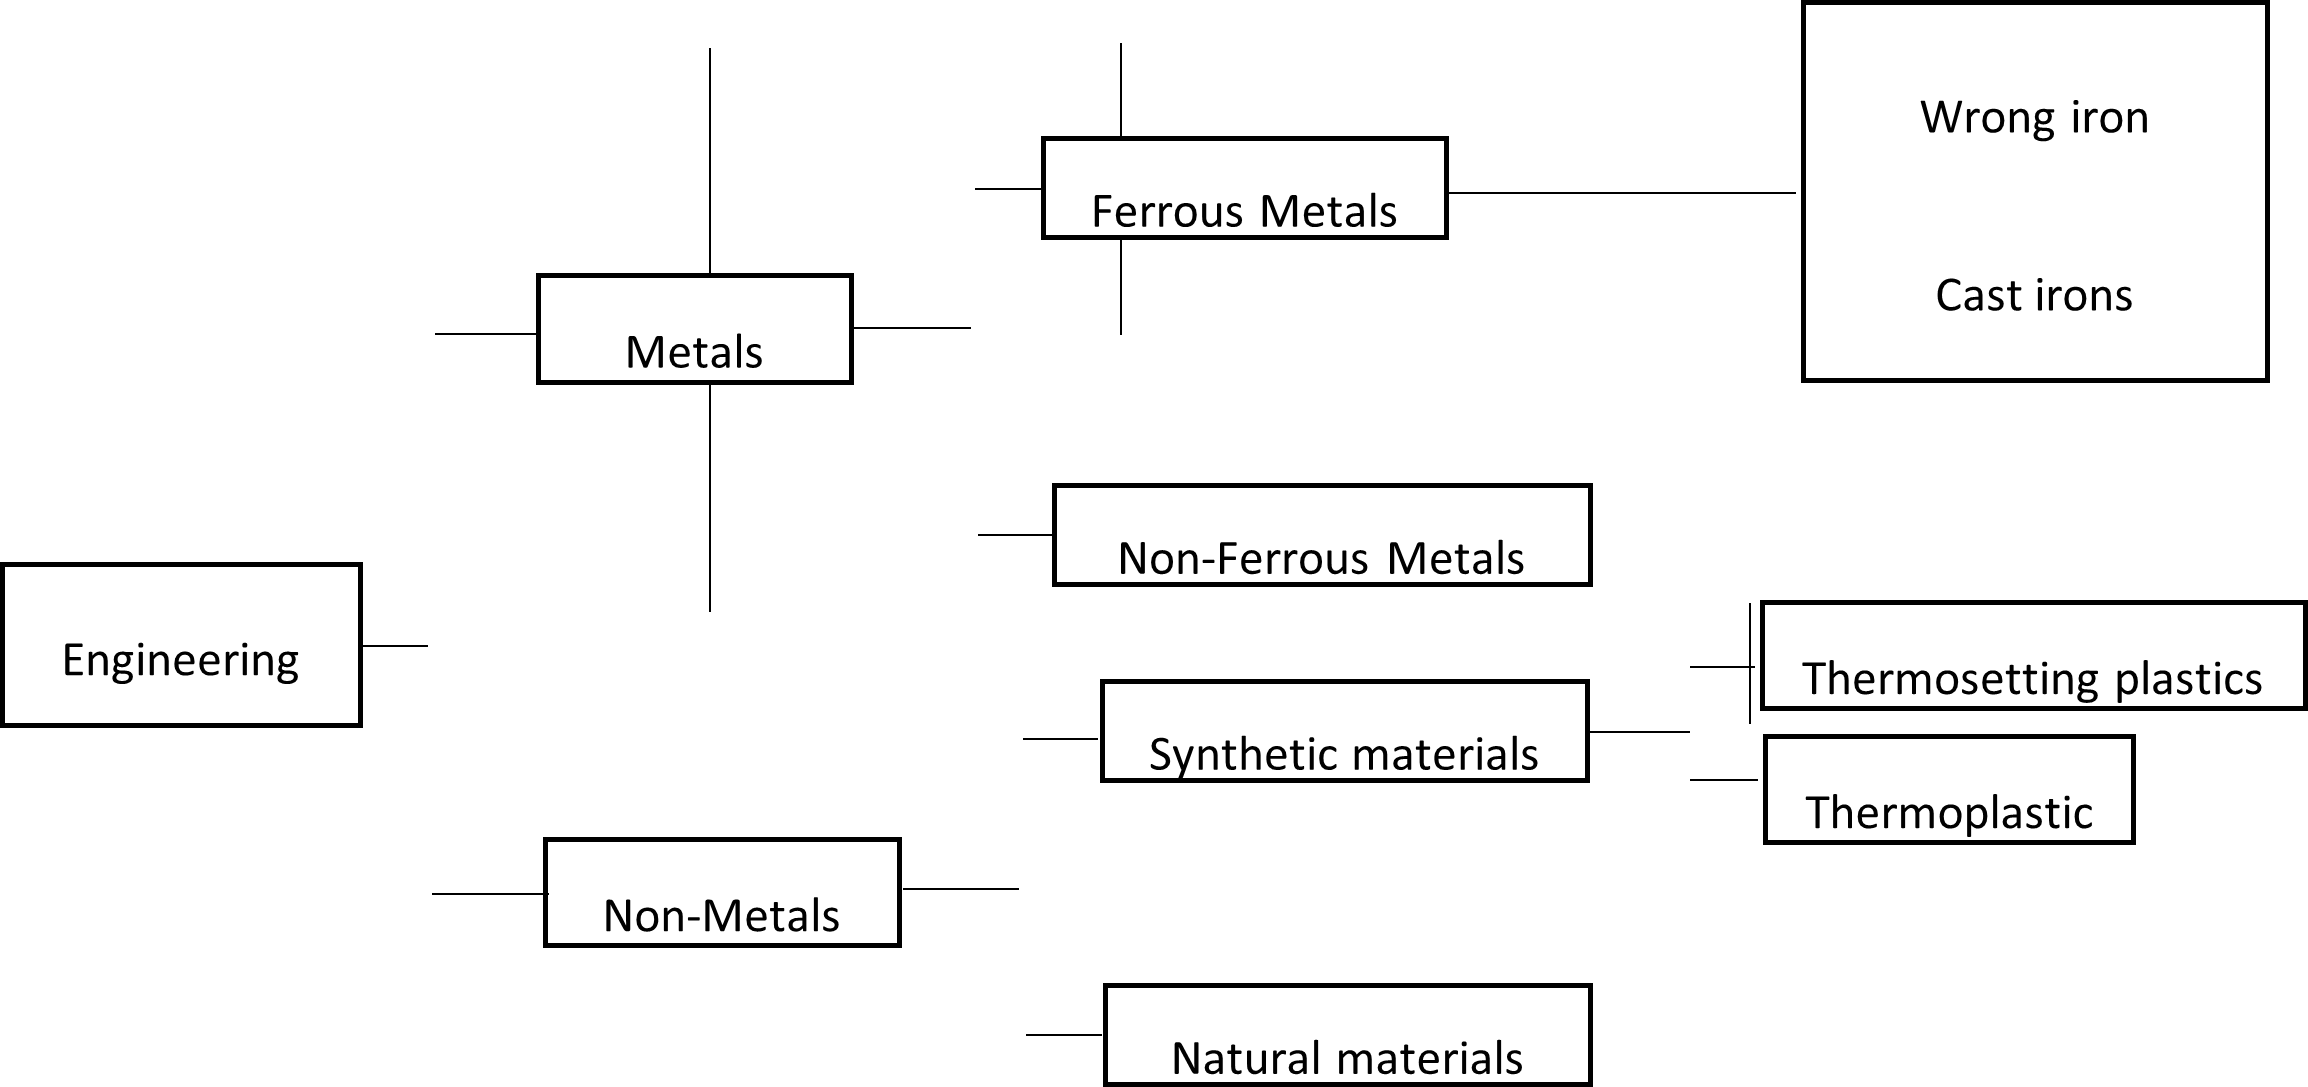
\includegraphics[width=\textwidth]{materials_classification.png}
    \caption{Engineering materials classification \cite{timings2008fabrication}}
    \label{ch3:figure:materials}
\end{figure}

Material selection is not a new era, it is a large and traditional branch of engineering materials. Moreover, it requires technical expertise. Material properties can be decisive when evaluating the storage facility material of construction. Material property is defined as an intensive property of a material that is not influenced by the amount of the material \cite{mcarthur2004engineering}. Typically, these are the properties we can measure or test. These properties can continuously interfere with the product stored in the storage tank; hence it is crucial to thoroughly comprehend them. There are several properties of materials, but in the present study, the following broad properties: physical and mechanical will be carefully investigated, with an effort of improving these properties, thus ensuring the compatibility of the storage facility material of construction with \acrshort{afff} concentrate.

It is vital to decide whether you are investigating the properties of the material or an object, as this could cause a contradiction. For example, you should decide whether you are identifying the properties of the storage facility or the properties of the material it is constructed of. Properties such as the shape and mass of the object (storage facility) may vary, even when they are constructed of the same material. It is for the same reason that it is assumed that the construction structure of the storage facility can have an impact on the performance parameters of \acrshort{afff}.  In other instances, material properties can be improved by processes such as mixing, heating, and cooling (heat treatment). This may be useful as the improved properties may yield better performance. For this reason, it is of great significance to evaluate the surrounding environmental factors that may change the initial material properties, thus affecting the \acrshort{afff} concentrate in that process.

Traditionally, storage facilities were constructed using metallic materials. However, in the last decade, researchers have developed specialized non-metallic materials in the form of composite materials to enhance materials that are utilized to construct storage facilities. These exceptional materials have diverse and combined properties that produce even better performance for storage facilities. Nevertheless, these advanced materials have some limitations and challenges that are notable during the specialized manufacturing technique.

This section gives an overview of the current materials that are used to construct the \acrshort{afff} concentrate storage facilities. First, the material characteristics and properties of metallic materials are discussed and carefully evaluated. Since non-metallic materials are gradually emerging, then their properties and limitations are also discussed. Finally, the four common materials used in the present study are specified, and various concerns regarding these materials are analyzed to identify and close the possible gaps that currently exist.

\subsection{Metallic materials}
Metallic materials are a significant part of engineering materials and have been extensively studied and used for a variety of purposes.  In material sciences, metallic materials are inorganic substances that usually contain a combination of metallic elements, which may also contain small amounts of non-metallic elements \cite{ali2020empirical}. The typical combination of metallic elements could be metals such as gold, iron, titanium, aluminium, etc. The small amount of non-metallic could be elements such as carbon, nitrogen, oxygen, etc \cite{hench2005biomaterials}. In physical sciences, there are 118 elements on the periodic Table, and 86 of these belong to the metallic group \cite{ali2020empirical}. All these 86 metals have diverse characteristics, and a limited number of these can be significantly used for engineering and other purposes.

In the last century, scientists have been working tirelessly to significantly understand these types of materials to develop efficient techniques that will aid in the optimization of metallic materials. With that being said, over the last 70 years, scientists have developed new techniques for producing various materials with enhanced properties to those of natural materials \cite{ali2020empirical}. To date, numerous metallic materials such as gold and copper mostly rely on these new techniques to yield effective performance. Consequently, metallic materials are rarely utilized as authentic elements, thus they are usually blended with other elements to form an alloy \cite{hench2005biomaterials}. Many storage facilities are constructed using alloy metals due to their distinctive characteristic properties.

The metallic materials are broadly classified as ‘ferrous and non-ferrous’ \cite{ali2020empirical}. Ferrous metals are those that contain iron (Fe) elements within them, while non-ferrous metals do not contain any iron element. In the present study, only ferrous metals will be discussed. Ferrous metals are vital in the present study, as mild and stainless steel materials will be experimentally evaluated when used as an \acrshort{afff} storage facility.  Mild and stainless steels are regarded as ferrous metals due to the presence of iron in their structure. Usually, ferrous metals suffer from the ‘corrosion phenomenon’ due to the presence of iron. Ferrous materials constitute more than 50\% of the metallic materials section \cite{ali2020empirical}. Furthermore, these materials (ferrous) are useful in numerous applications as they meet the various service requirements of our modern and complex society.

While scientists have managed to develop efficient techniques for producing metals, it was of great importance to understand the relationship between structural elements of the materials and their properties. In the textbook ‘engineering materials science’ by Mcarthur and Spalding \cite{mcarthur2004engineering}, the microstructure is defined as the arrangement of crystals (or grains) of the different phases. Hence, these are observed when a polished section of a piece of the material is viewed at high magnification through a microscope \cite{molabe2018determining}. The chapter on metallic materials has been studied extensively. As a consequence, it has been experimentally proven over the past decades that the properties of metallic materials are interrelated with the microstructure of the material itself. This is evidence that the properties can be enhanced by altering the relative proportions of the micro-constituents (or phases). Phases are identified by their unique crystal structures, composition, and properties \cite{mcarthur2004engineering}.

Liquid storage facilities are critical in ensuring that the properties of the stored products are well maintained. Metallic materials have offered numerous and diverse benefits when utilized as liquid storage facilities. However, in other instances horrible incidences that result in storage facility catastrophic failure occur. This proves that although metallic materials are beneficial, there are still gaps that exist, probably in the metal production optimization, enhancing of natural properties, and relevant materials selection. There are relatively three factors that may influence the choice of metals and alloys when used as an \acrshort{afff} storage facility:

\begin{itemize}
    \item Mechanical, physical, chemical, and thermal properties.
    \item Degradation of the material.
    \item Compatibility with the product to be stored, which is \acrshort{afff} for the present study.
\end{itemize}

Understanding relevant material selection will aid in easing the enhancement of the properties of metallic materials. This will be more useful in metallic materials that are widely utilized to construct the storage facility for storing \acrshort{afff} concentrate. 

\subsection{Metalic bonding}
In general, the term ‘bonding’ can be described as the action of joining two or more things firmly, especially employing adhesive, heat, or chemical bonds \cite{soler2000metallic}. In materials and science, there are three types of bonding: covalent, ionic, and metallic bonding. For the present study, the focus will be on evaluating and comprehending metallic bonding.

In the early 1900s, Paul Drüde discovered the metallic bonding theory by modelling metals as a mixture of atomic cores (positive nuclei + inner shell of electrons) and valence electrons \cite{sinex2017general}. Metallic bonding can be described as the type of chemical bond formed between positively charged atoms in which the free electrons are shared among a lattice of cations \cite{lepetit2017topological}. In contrast, covalent and ionic bonds form between two distinct atoms. Metallic bonding in the major type of chemical bonding that forms between metal atoms. Figure \ref{ch3:figure:bonding} shows how a metallic bond occurs.

\begin{figure}[H]
    \centering
    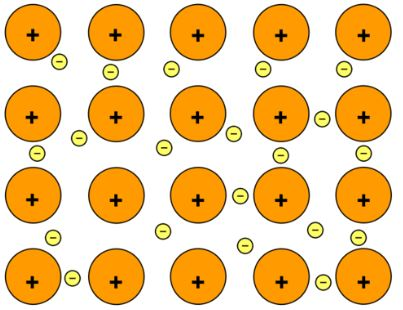
\includegraphics[width=.5\textwidth]{metalic_bonding.jpg}
    \caption{Metalic bonding: Positive atomic nuclei (orange circles) surrounded by delocalized electrons (yellow cirlces) \cite{soler2000metallic}.}
    \label{ch3:figure:bonding}
\end{figure}


Metallic bonds are commonly noticed in natural metals, alloy metals, and some metalloids. For instance, graphene (an allotrope of carbon) usually reveals two-dimensional metallic bonding \cite{lepetit2017topological}. It should be noted that metals, including natural ones, are not limited to metallic bonding. Thus, they have the capability of forming other types of chemical bonds within their atoms.

All atoms contain a small nucleus of neutrons and protons these are surrounded by orbiting electrons \cite{hench2005biomaterials}. Distinct atomic models can be significantly used to describe different properties of the overall material. As previously stated, one beneficial model of a metal is a repeating structure of metallic ions, which are surrounded by a ‘sea’ of electrons, see Figure \ref{ch3:figure:bonding}. It is the ‘free electrons’ that critically determine the thermal and physical properties of the metallic material \cite{hench2005biomaterials}. Alternatively, several mechanical properties of metallic materials can be better understood by considering atoms to behave like ‘hard spheres’ \cite{hench2005biomaterials}. This is vital in the present study as this will be used as a benchmark in improving the properties of alloy metals that are commonly utilized as \acrshort{afff} storage facilities.

When atoms are behaving like hard spheres, they are relatively bonded together by an attractive force \cite{lepetit2017topological}. However, this type of bonding is very weak, which is the reason why metals have a crystalline structure where atoms are significantly arranged in a dense, regular, and repeating manner. The atoms of various metals are significantly arranged in various crystal structures \cite{hench2005biomaterials}. Atoms in metallic materials can be relatively arranged in four (4) different ways these include face-centred cubic (\acrshort{fcc}), \acrfull{hcp}, body-centred cubic (\acrshort{bcc}) and tetragonal. A typical example may include a pure metal such as aluminium (Al) in which atoms are relatively arranged in \acrshort{fcc} at room temperature \cite{hench2005biomaterials}, as shown in Figure \ref{ch3:figure:aluminium}.
 
\begin{figure}[H]
    \centering
    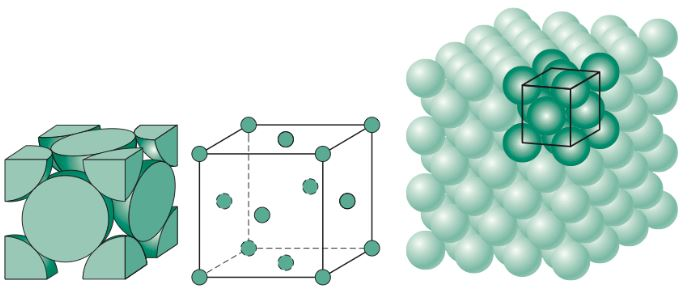
\includegraphics[width=\textwidth]{aluminium_crystal_structure.jpg}
    \caption{Crystal structure of aluminium metal (Al) at room temperature \cite{hench2005biomaterials}.}
    \label{ch3:figure:aluminium}
\end{figure}

The mentioned crystal structures are determined at room temperature.  However, the transition in the crystal structure is much more possible in several metals. This transition varies with the temperature to which the metal is exposed \cite{callister2018materials}. For example, metals such as pure iron may reveal two different crystal structures. At room temperature it reveals \acrshort{bcc}, but when the temperature is constantly increased towards a melting point (912-1394℃), its crystal structure changes to \acrshort{fcc}. Further increasing the temperature to about 1538 ℃ will result in reverting the crystal structure to \acrshort{bcc} \cite{ali2020empirical, molabe2018determining}. For alloy metals, the transition in the crystal structure can be achieved by adding an element with a different crystal structure. The transition in alloy metals will be evaluated in detail in Section \ref{ch3:anchor:section:morphology}. Table \ref{ch3:table:structure} shows the atom arrangement in a crystal structure of some commonly used pure metals.

\begin{table}[H]
\caption{Crystal structure for popular metals, at room temperature \cite{hench2005biomaterials}.}

\begin{tabularx}{.8\textwidth}{ XX }
    \hline
    Metal & Crystal structure \\
    \hline
    Aluminum & FCC \\
    Chromium & BCC \\
    Copper & FCC \\
    Gold & FCC \\
    Iron & BCC \\
    Silver & FCC \\
    Nickel & FCC \\
    \hline
\end{tabularx}

\label{ch3:table:structure}
\end{table}

Several physical and mechanical properties of materials are determined by the metallic bonds and the arrangement of the atoms in the crystal structure. For example, when metallic material is heated to a melting point, the atoms have to gain sufficient energy to break free from the crystal structure \cite{hench2005biomaterials}. This is evidence that the properties of materials can be altered by altering the arrangement of atoms in a crystal structure. Moreover, the crystal structure significantly determines the ability of atoms to slip over one another during the deformation of metals \cite{callister2018materials}. This is especially true in ductile metals due to their ability to deform without easily breaking. These types of materials are commonly used to construct liquid storage facilities due to their crystal structure that yields exceptional properties.

\section{Mild steel the material}
\label{ch3:anchor:section:material}
Mild steel is a ferrous metal that contains a relatively low content of carbon, which usually ranges from 0.05\% to 0.25\% by weight \cite{callister2018materials}. Thus, it is also known as 'low-carbon steel.  Low-carbon steels consist primarily of ferrite rather than perlite \cite{li2018effect}. Metals containing carbon content from 0.30 to 2.0\% are typically referred to as higher carbon steel \cite{timings2008fabrication}. The addition of carbon content increases the strength of the steel. Consequently, steel materials having a carbon content higher than 2\% are often regarded as ‘cast-iron' \cite{callister2018materials}.  Mild steel is a popular metallic material that has been extensively used for many applications, including industrial storage facilities.

Although mild steel contains carbon, iron, and other elements in its composition, it nonetheless cannot be regarded as alloy steel. This is due to the extremely low amount of carbon and other alloying elements it contains; thus, these elements are insufficient to produce alloy steel. The relatively low amount of carbon and other alloying elements in the composition of mild steel results in diverse properties when compared to higher carbon and alloy steels \cite{timings2008fabrication}. The high content of iron and ferrite in the composition of mild steel means that it is magnetic \cite{li2018effect}.

Low-carbon steels are generally useful in liquid storage facility construction, due to their compatible properties. In particular, mild steel is one of the most commonly used tank construction materials. It is popularly known for its ductility and can be made from readily available natural materials. The low cost of this metal makes it beneficial to numerous industries in terms of economic.

The low-carbon steel setback to date has been corrosion, which causes more serious deterioration problems in storage facilities\cite{erami2019carboxamide}. Various coatings have been developed over the past decade, aiming to mitigate this problem. The other major concern regarding low-carbon steels is that it is nearly impossible to alter some of the mechanical properties through heat treatment \cite{callister2018materials}. Moreover, low-carbon content means that mild steel has very few alloying elements to prevent dislocation in the crystal structure, resulting in less tensile strength than high-carbon and alloy steels \cite{callister2018materials}.

This section provides and evaluates mild steel as a material and also as an object (storage facility). The scope of this section includes the evaluation of the current properties and their impacts on the \acrshort{afff} storage facility. Similarly, the understanding of the microstructure of low-carbon steels to develop useful strategies to improve the properties and compatibility of this metallic material is essential for the present study. The machinability of low-carbon steels is evaluated. Furthermore, the corrosion concerns are discussed, and common methods to prevent this are briefly discussed. Finally, the heat treatment processes that are commonly used to enhance the properties are also closely assessed. This will aid in understanding the gaps in the optimization of the properties.

\subsection{Useful properties} 
As previously stated, the material property is a comprehensive property that is not dependent upon the amount or size of the material \cite{kabir2020critical}. These are the quantitative parameters that are measurable/tested and observed when a load is applied. As a consequence, these properties are significantly determined by the composition and crystal structure of the material. Thus, it is vital to understand the arrangement of atoms in the crystal structure. Furthermore, before any material is selected for a certain application, the properties should be immensely understood to ensure compatibility with the application utilized.

Mild steel has a variety of properties that makes it beneficial for several applications and these are detailed in Figure \ref{appendix:carbon_steel_properties} in the appendices. These properties can be broadly grouped into mechanical and physical properties \cite{kabir2020critical}. These two properties are vital determinants for which metal is considered to be compatible with a given application. In almost every instance, mechanical properties are interdependent, meaning high performance in one category may be achieved with lowering performance in other categories \cite{kabir2020critical}. For example, the low content of carbon in mild steel means that this metallic material is more ductile when compared to alloy steel.

For low-carbon steels, ductility indicates that they can be formed into the desired shape at any temperature without major difficulties \cite{dong2005deformation}. Figure \ref{ch3:figure:carbon} shows how the carbon content of plain carbon steel affects the properties of the steel. Referring to Figure \ref{ch3:figure:carbon} it can be observed that altering carbon content in plain carbon steels has an impact on the properties. Consequently, when the carbon content has increased, the ductility of the steel materials is relatively decreased. Moreover, the strength and hardness are remarkably increased, which results in the transition from ductile to brittle \cite{abou2001mechanical}. For liquid (\acrshort{afff}) storage facilities, ductility is one of the significant properties. This property means that the storage facility can be rolled or joined using various mechanical fabrication methods mentioned in Section 4.3.1, without having major concerns.
 
\begin{figure}[H]
    \centering
    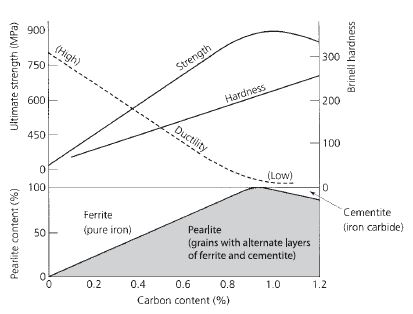
\includegraphics[width=.65\textwidth]{effect_of_carbon_content.jpg}
    \caption{Effect of carbon content on the properties of plain carbon steel \cite{timings2008fabrication}.}
    \label{ch3:figure:carbon}
\end{figure}

Another critical parameter for storage facilities constructed of mild steel is thermal conductivity, which falls under physical properties. In the textbook, ‘heat transfer: a practical approach’ by Cengel \cite{cengel1998heat} thermal conductivity is defined as a measure of the quantity of heat that flows through a material. In the present study, the storage facility does not necessarily need to be constructed with materials that have a high thermal conductivity. However, achieving this is somehow difficult, due to the diverse properties a material can have.

Mild steel has a thermal conductivity of 64.86 $\nicefrac{W}{m.K}$ at most \cite{cengel1998heat}. This is quite less when compared to other steels but can be considered high for applications that do not require heat transfer. At extremely high temperatures, heat may be transferred to the product inside the storage tank and may influence the viscosity of the product. For the present study, heat transfer is not a concern, due to the environment (atmospheric), the storage facility is located on. However, when looking at this from another perspective, it can cause problems along the time. When the storage facility is continuously exposed to high-temperature environments, heat can be gradually transferred until it causes some notable problems to \acrshort{afff} solution. To reduce heat transfer, insulating materials are usually utilized, but they however do not eliminate the problem completely. As a consequence, it is vital to understand the environmental factors that may associate with the properties of the material on the location of the storage facility.

There are normally three means of transferring heat namely conduction, convention, and radiation. Conduction involves heat transfer through solid materials, convention is associated with heat transfer between a solid surface and a gas or liquid that is in motion, while radiation is the energy emitted by the matter in the form of electromagnetic waves \cite{cengel1998heat}. In the case of \acrshort{afff} storage facilities, heat transfer by conduction is of great interest, as this is the possible scenario in this circumstance.   

For the worst situation, the total heat energy that can be transferred to the storage facility, hence \acrshort{afff} concentrate as a result of the surround atmosphere (radiation) can be calculated using the energy balance equation as follows:

\begin{equation}
    Q_c = m \times C_p \times \Delta T
\end{equation}

\begin{doublespace}
\noindent Where, \\
$Q_c\ is\ the\ amount\ of\ net\ heat\ transfer\ to\ the\ system\ in\ J$ \\
$m\ is\ the\ mass\ of\ a\ material\ in\ kg$ \\
$C_p\ is\ the\ specific\ heat\ capacity\ in\ \nicefrac{kJ}{kg.^\circ C}$ \\
$\Delta T\ is\ the\ temperature\ difference\ of\ surfaces\ in\ ^\circ C$ \\
\end{doublespace}

When the total heat energy that is being transferred to the storage tank holding \acrshort{afff} is known, it is now vital to estimate the rate at which this heat energy is being transferred. This is critical in predicting whether the composition of \acrshort{afff} concentrate is being affected by the heat that is transferred to the storage facility by conduction. The equation for calculation of conduction heat transfer rate is known as Fourier’s Law of Heat Conduction and is given by:

\begin{equation}
    Q_c = -k \times A \times \frac{\Delta T}{\Delta r}
\end{equation}


\begin{doublespace}
\noindent Where, \\
$Q_c\ is\ the\ conductive\ heat\ transfer\ rate\ in\ W$ \\
$k\ is\ the\ thermal\ conductivity\ of\ thematerial\ in\ \nicefrac{W}{m.^\circ C}$ \\
$A\ is\ the\ cross-sectional\ area\ in\ m^2$ \\
$\Delta T\ is\ the\ temperature\ diifference\ of\ surfaces\ in\ ^\circ C$ \\
$\Delta r\ is\ the\ distance\ separating\ the\ surfaces\ in\ m$ \\
\end{doublespace}
In heat transfer, positive heat conduction means that heat is flowing into the body in question, and negative heat conduction represents heat leaving the body. Heat transfer has been applied in various research fields mainly to increase the heat transfer rate, decrease heat transfer rate and keep the temperature in a certain range. For the present study, the focus is to ensure a decrease in the rate of heat transfer, so that it will not suddenly change the composition of \acrshort{afff}, thus influencing its firefighting performance.  

Another property of interest for the present study is the effect of corrosion on steel. Corrosion is the process of decay of a material (usually ferrous metals) caused by a chemical reaction with its environment \cite{islam2018effects}. \acrshort{afff} concentrate is generally not a corrosive type of liquid. However, mild steel contains about 98\% iron in its composition, which is significantly high and makes it to be considered a corrosive ferrous metal.  The corrosion phenomenon is usually prevented in several ways, and these will be discussed in detail in Section \ref{ch3:anchor:section:effects}.


\section{Stainless steel the material} 
Stainless steels are ferrous metallic materials that contain a minimum of 10.5\% of chromium and about 8\% of nickel as the main alloying element \cite{sourmail2005stainless}. All the alloying elements have a significant role in the stainless steel family. Chromium element forms a protective self-healing oxide film, which greatly improves the corrosion resistance of stainless steel \cite{molabe2018determining}. Large amounts of nickel contribute to both heat and corrosion resistance \cite{george2002introduction}. However, depending on the percentage of nickel added, it also contributes to high strength and excellent toughness. Other relevant elements are often added to enhance the properties of stainless steel. It is these alloying elements that make stainless steel to be generally more expensive than carbon steel.

The classification of stainless steel is based on the nature of its metallurgical structure \cite{bhadeshia2017steels}. As previously stated in Section \ref{ch3:anchor:section:material}, the metallurgical structure is the arrangement of the atoms making up the grains of the steel. The microstructure is formed based on the chemical composition of the steel. With an appropriate combination of alloying elements that results in a unique microstructure, stainless steels can be fully austenitic, and a mixture of ferrite and austenite (duplex), fully ferritic or martensitic \cite{bhadeshia2017steels}. These four possible microstructure phases are shown in Figure \ref{ch3:figure:steel_phase}. These categories of stainless steel are obtained under specific cooling conditions, and all are beneficial for various applications.
 
\begin{figure}[H]
    \centering
    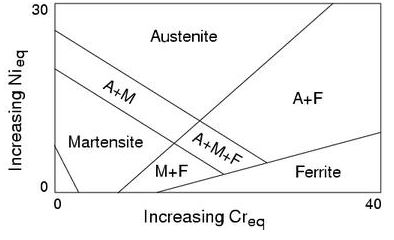
\includegraphics[width=.65\textwidth]{stainless_steel_phase.jpg}
    \caption{Stainless steel phase diagram as a function of chromium and nickel equivalents at room temperature \cite{bhadeshia2017steels}.}
    \label{ch3:figure:steel_phase}
\end{figure}

In the present research work, duplex stainless steel is of great significance. As can be seen in Figure \ref{ch3:figure:steel_phase}, the duplex contains a combination of austenite and ferrite, approximately 50\% of each. It is more beneficial and extensively used in liquid storage facilities, as it yields a combination of properties. This is due to a large amount of chromium and less nickel content presence, which results in corrosion resistance, high strength, and excellent toughness \cite{gunn1997duplex}. The weighed composition of duplex stainless steel is detailed in Figure \ref{appendix:duplex_stainless_steel_properties} on appendices. The less content of nickel in duplex stainless steel implies that duplex is relatively inexpensive compared to other classes \cite{sourmail2005stainless}. The two-phase mixture also reduces the risk of intergranular attack; for the same reason, they are not prone to solidification cracking during welding \cite{sourmail2005stainless}. Figure \ref{ch3:figure:weight} shows the comparison of the weight percentage of \acrfull{cr}, \acrfull{ni}, and \acrfull{mo} in duplex and austenitic stainless steel.
 
\begin{figure}[H]
    \centering
    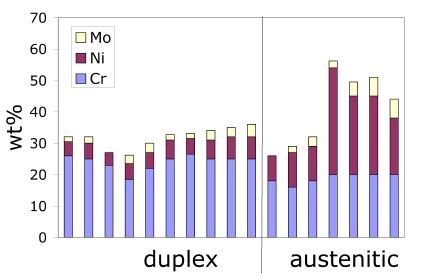
\includegraphics[width=.65\textwidth]{weight_percentages.jpg}
    \caption{Weight percentage of Cr, Ni, and Mo in duplex and austenitic steels \cite{sourmail2005stainless}.}
    \label{ch3:figure:weight}
\end{figure}

In general, stainless steel is an excellent metallic material that has several useful properties which are shown in Figure \ref{appendix:stainless_steel_properties} in the appendices. Consequently, this type of steel offers numerous benefits for various applications. Although stainless steel is popularly known for excellent corrosion resistance, reports in recent years have suggested otherwise \cite{karayan2014weld}. Corrosion in stainless steel often occurs unexpectedly on the welded joints, which then affects the product that is stored, particularly in welded storage tank applications. Another concern for stainless steel is the difficulty in machinability \cite{grzesik2008advanced}. Fabricating or manufacturing stainless steel is not an easy task, due to the elements it contains. All these concerns are greatly dependent on the microstructure of the material, and the possible optimization methods will be discussed in Sections \ref{ch3:anchor:section:morphology} and \ref{ch3:anchor:section:treatment} respectively.

\section{Effect of corrosion on steels}
\label{ch3:anchor:section:effects}
Corrosion is an integrative and critical subject of matter that has numerous half-truths and myths, which exist to date \cite{mcarthur2004engineering}. These are continuously occurring due to ignorance when it comes to the science of corrosion.  Corrosion is a phenomenon that commonly affects ferrous metals due to the presence of iron. In corrosion science, corrosion is defined as the deterioration of a substance or its properties due to interactions between the substance and its environment \cite{chigondo2016recent}.

In recent years, corrosion has become a vital matter in liquid storage facilities, especially in acidic liquids. Corrosivity is generally measured by either pH or the rate of steel corrosion \cite{marzorati2018green}. When the aqueous concentrate has a Ph less than or equal to two, or more than or equal to 12.5, it is considered to be corrosive \cite{marzorati2018green}. As a consequence, corrosion is generally not a concern in storage facilities containing \acrshort{afff} concentrate since it has an approximate Ph value of 7-8.5. However, the storage facility can nonetheless suffer from corrosion due to the surrounding environment. In the present research, a storage facility containing \acrshort{afff} concentrate is continuously exposed to the corrosive atmospheric environment (Durban, South Africa) due to the near sea. Figure \ref{ch3:figure:ph} shows the corrosive Ph level of an aqueous concentrate.
 
\begin{figure}[H]
    \centering
    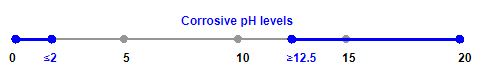
\includegraphics[width=.8\textwidth]{aqueous_solution_ph_scale.jpg}
    \caption{Ph scale for aqueous solution \cite{marzorati2018green}.}
    \label{ch3:figure:ph}
\end{figure}

Although there is a lack or little knowledge of the corrosion phenomenon, some researchers have made significant efforts to understand it. The material is initially selected due to the desired properties. However, some recently published literature suggests that corrosion has a degrading effect on mechanical properties. Mahmoodian et al. \cite{li2018effect} conducted a study that concluded that corrosion can lead to a reduction of the thickness of the storage facilities, and thus in the reduction of yield strength, ultimate strength, and ductility on low carbon steels.  Marcus \cite{protopopoff2011surface} further stated that the reduction of these properties is due to hydrogen accumulation within the steel, which is known as \acrfull{he}. Besides, this accumulation of hydrogen results in a sudden reduction in the ductility of steel. Figure \ref{ch3:figure:degradation} shows the process of mechanical properties degradation due to corrosion.
 
\begin{figure}[H]
    \centering
    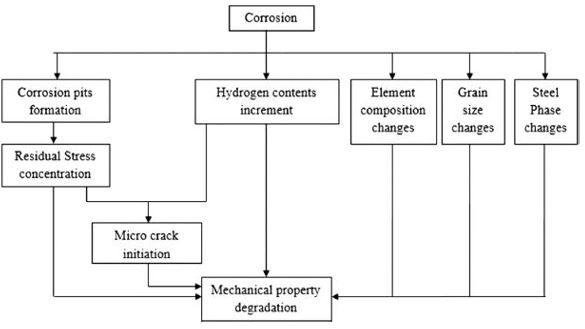
\includegraphics[width=\textwidth]{process_of_mechanical_properties.jpg}
    \caption{Process of mechanical properties degradation due to corrosion \cite{protopopoff2011surface}.}
    \label{ch3:figure:degradation}
\end{figure}

In more detail, corrosion occurs when there is a combination of oxygen reduction and hydrogen evolution reactions, as shown in equations (\ref{ch3:equation:acid} – \ref{ch3:equation:neutralalkaline}) \cite{li2018effect}.  Consequently, during these reactions, atomic hydrogen is released. It then eventually accumulates at the defects within the steel, forming molecular hydrogen. Finally, the molecular hydrogen results in the increase of inside pressure, and eventually micro-cracking initiations, which consequently degrades the mechanical properties of steel \cite{whitman1924effect}.

Oxygen Reduction Reaction (ORR)

\begin{equation}
    \frac{1}{2}0_2 + 2H_3O^{+2e \rightarrow 3H_2OAcid}
    \label{ch3:equation:acid}
\end{equation}

\begin{equation}
    \frac{1}{2}O_2 + H_2O + 2e \rightarrow 2OH^{-Neutralalkaline}
\end{equation}

Hydrogen Evolution Reaction (HER)

\begin{equation}
    H_3O^{++e \rightarrow \frac{1}{2}H_2 + H_2OAcid}
\end{equation}

\begin{equation}
    H_2O + e \rightarrow \frac{1}{2}H_2 + OH^{-Neutral,alkaline}
    \label{ch3:equation:neutralalkaline}
\end{equation}

Based on Equations (\ref{ch3:equation:neutralalkaline} - 3.9), it is sensible to believe that corrosion changes the elemental composition of the steel. However, few papers focus on monitoring the changes in element composition during corrosion. Corrosion may also result in the degradation of mechanical properties by changing three microstructural features: (1) grain size, (2) phase composition, and (3) formation of corrosion pits \cite{li2018effect}. Presumably, corrosion is interrelated with the microstructure of the material. For example, grain size reduction causes more hydrogen absorption within steel \cite{li2018effect}. However, there are several limitations to existing Research. To begin with, the hydrogen embrittlement phenomenon has been mainly carried out for \acrfull{hsla} and stainless steel \cite{li2018effect}. As a consequence, extensive research should be conducted to determine the degradation mechanism of mechanical properties due to corrosion, at both macro and micro levels.

Many researchers have been interested in the corrosion phenomenon, thus over the years, there have been several ways developed to prevent corrosion. Corrosion can occur in many ways, thus it is also significant to understand different types of corrosion and evaluate the corrosion of interest. Stainless and mild steel are the metallic materials of interest in the present study; thus, it is vital to understand the different ways in which corrosion occurs in these two metallic materials. In this way, it is possible to optimize the current methods that are utilized to prevent corrosion, focusing precisely on the corrosion of interest.

As previously stated, several half-truths and myths regarding corrosion exist. Stainless steel is popularly known for resisting corrosion due to the presence of a chromium element in its composition. However, these are myths and half-truths due to the incidences that have proven that stainless steel can suffer from corrosion. This is usually the case on welded products. In contrast, mild steel is well known for suffering from corrosion, this is due to the lack of corrosion-protecting alloying elements such as chromium \cite{hackerman1987theory}. However, corrosion prevention is more practical than making an effort to eliminate it. A stainless steel storage facility that has suffered from corrosion on welded joints is shown in Figure \ref{ch3:figure:tank}.
 
\begin{figure}[H]
    \centering
    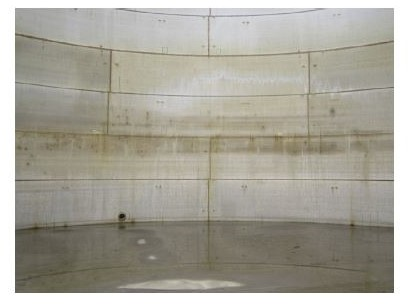
\includegraphics[width=.55\textwidth]{storage_tank.jpg}
    \caption{Storage tank that corroded on welded joints \cite{karayan2014weld}.}
    \label{ch3:figure:tank}
\end{figure}

\subsection{Types of corrosion} 
The tendency of a metal to corrode depends upon the crystal structure of the metal, its composition as formed during alloying, and the temperature for deformation of a single metal surface developed during fabrication \cite{sourmail2005stainless}. The environment plays a key role in the corrosion of the material; thus, it can vary with the environment to which the substance is exposed. Consequently, this makes it complex to comprehend the corrosion mechanism. Corrosion can be caused by diverse factors that include the reactivity of metal, the presence of impurities, the presence of air, moisture, gases like sulphur dioxide, and carbon \cite{sourmail2005stainless}. Therefore, corrosion protection and prevention are significantly aimed at addressing these factors. There are various types of corrosion, and it is vital to understand which corrosion you are faced with. The different types of corrosion which depend upon the environment surrounding the material, type of material, or chemical reaction are briefly described in Table \ref{ch3:table:corrosions}.

\begin{table}[H]
\caption{Types of corrosion \cite{chigondo2016recent}.}

\centering
\renewcommand{\arraystretch}{2}
\begin{tabularx}{\textwidth}{>{\hsize=0.65\hsize}X >{\hsize=1.35\hsize}X}
    \hline
    Type of corrosion & Description \\
    \hline
    Uniform corrosion & Deteriorates the whole surface of the metal and makes the surface thin. \\
    Galvanic corrosion & Occurs with an electrolyte with metal having different values of electrical potentials. \\
    Pitting corrosion & Occurs because of the random attacks on particular parts of the metal's surface to form pits. The pit acts as an anode, while the undamaged part of the metal is the cathode. \\
    Stress corrosion cracking & A complex form of corrosion which arises due to stress and  corrosive environment. \\
    Corrosion fatigue & A combination of cyclic stress and corrosion.  \\
    Intergranular corrosion & Corrosion occurs on or near the grain boundaries of a metal.  \\
    Crevice corrosion & Concentration cell corrosion due to the trapping of corrosive liquid  between the gaps of the metal. \\
    Filiform corrosion & Concentration cell corrosion on metallic surfaces coated with a thin  organic film. \\
    Erosion corrosion & Flow-assisted corrosion which is due to the movement of corrosive  liquids on metal surface. \\
    Fretting corrosion & A form of corrosion which shows the combined effect of corrosion and  fretting of metal. \\
    \hline
\end{tabularx}

\label{ch3:table:corrosions}
\end{table}

In the present study, the focus is on stress corrosion cracking/atmospheric corrosion. As can be observed in Table \ref{ch3:table:corrosions}, stress corrosion cracking is a complex form of corrosion which arises due to the stress and corrosive atmosphere. However, the cracking of the storage facility due to stresses is not a concern in the present study, thus the focus is particularly on the corrosive atmospheric environment.

\subsubsection{Atmospheric corrosion}
Atmospheric corrosion is a naturally occurring chemical deterioration of a material due to a reaction with the environment, especially with oxygen. The extent of deterioration of a ferrous metal depends on the chemical composition and grain structure of the material. For example, when iron is exposed to an industrial atmosphere for a long period, iron oxide, also known as rust, forms on the surface, as shown in Figure \ref{ch3:figure:corrosion} \cite{mcarthur2004engineering}. The rust is very porous to oxygen and water in the atmosphere, and consequently, the corrosion process continues until the metal is entirely consumed \cite{protopopoff2011surface}.  Atmospheric corrosion generally occurs in three various environments rural, industrial, and marine. For the present study, the industrial environment is the benchmark since the storage facility is located in an industrial environment. Figure \ref{ch3:figure:corroded} shows the storage facility, which was initially protected from corrosion yet ended up suffering from rural atmospheric corrosion.

\begin{figure}[H]
    \centering
    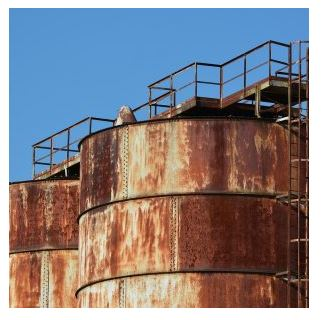
\includegraphics[width=.55\textwidth]{corrosion_of_storage_facilities.jpg}
    \caption{Atmospheric corrosion of storage facilities in industrial environment \cite{chigondo2016recent}.}
    \label{ch3:figure:corrosion}
\end{figure}
 
\begin{figure}[H]
    \centering
    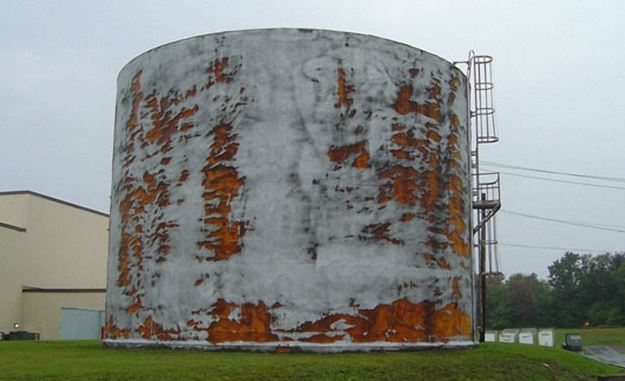
\includegraphics[width=\textwidth]{corroded_storage.jpg}
    \caption{Corroded storage facility \cite{protopopoff2011surface}.}
    \label{ch3:figure:corroded}
\end{figure}

Atmospheric corrosion is one of the most common types of corrosion, which is affected by several environmental factors. It commonly affects infrastructure, transportation, energy, and other industries \cite{pei2021understanding}. Over the decades, research has shown that contributing environmental factors affecting the outdoor atmospheric corrosion rate include temperature, \acrfull{rh}, atmospheric pollutants (commonly sulphur dioxide and chlorides), and wind \cite{abou2001mechanical, islam2018effects}. It is difficult to individually analyse the impact of these factors due to the existence of complex interactions between them.

In the past years, several researchers have made significant efforts in analysing the influence of a single factor on atmospheric corrosion. Cai et al. \cite{cai2018influence} studied the effects of \acrshort{rh}, temperature, sulfur dioxide, and chlorides on short-term corrosion behaviour in a dynamic environment. They demonstrated that \acrshort{rh} is the most influential factor in corrosion, and the temperature is secondary. The effect of \acrshort{rh} can be reflected by the \acrfull{tow} according to ISO9223 by the \Acrfull{iso} \cite{cengel1998heat, islam2018effects}. In 2020, Pei et al. \cite{pei2021understanding} further investigated the environmental impacts of \acrshort{rh}, temperature, and rainfall on the initial corrosion behaviour of steels. The outcomes showed that rainfall is the most influencing factor in the initial atmospheric corrosion rate.  Moreover, \acrshort{rh} significantly influenced the corrosion of steels in low precipitation environments and non-rainfall periods.

The environmental conditions are natural; thus, they keep changing unexpectedly. With this regard, it becomes difficult to predict the effect of a dynamic environment on atmospheric corrosion. Nevertheless, a model that predicts corrosion loss as a function of environmental parameters and exposure time is required. Cai et al. \cite{cai2018influence} suggested that to develop a model that will be effective in a dynamic environment, firstly, a corrosion kinetic model is required to predict the corrosion process over time. Then, a parametric method is necessary to describe the precise dynamic environmental factors. And finally, an accelerating model that describes the effects of environmental factors on the corrosion rate is essential to correlate the corrosion parameters with the environmental factors \cite{loto2019performance}. All these conditions exclude the effect of rainfall. The effect of acidic rain on the corrosion effect is very complex and thus is not understood fully \cite{pei2021understanding}. However, the use of corrosion (and environmental) monitoring techniques is highly desirable

\paragraph{Effects of atmospheric factors on corrosion} \hfill \\
Over the past years, researchers have successfully demonstrated that the atmospheric corrosion effect of environment on the metals comprises of three (3) main components parts: the effect of dry deposition of sulphur dioxide, the effect of dry deposition of chloride, and the effect of wet deposition of hydrogen ions (acid rain) \cite{cai2018influence}.

The amount of rainfall and acidity of the precipitation can be measured using a couple of existing exposure programs such as \Acrfull{micat} project, the \Acrfull{osd} program, and the \Acrfull{un/ece} program \cite{cai2018influence}. However, the existing data are limited, thus the quantitative models or programs cannot be successfully developed. Moreover, the lack of experimental data on the impact of hydrogen ions on atmospheric corrosion rate means that it is excluded from \acrshort{iso} 9223 \cite{protopopoff2011surface}. The factors affecting atmospheric corrosion are listed below.

\begin{itemize}
    \item \textbf{Relative humidity:} As stated previously, RH has a greater influence on the atmospheric corrosion of steel. The relationship between atmospheric corrosion rate and RH has been demonstrated by several researchers \cite{dong2005deformation, islam2018effects}. In addition, according to many researchers and scientists, the corrosion rate is directly proportional to RH \cite{dong2005deformation, islam2018effects}. Technically, when RH is increased in an environment the rate of atmospheric corrosion is also increased. RH is, however, independent of any other atmospheric factor. For example, when RH is increased typically from 75\% to 95\%, the rate of corrosion will increase regardless of the temperature \cite{sourmail2005stainless}
    
    \item \textbf{Temperature:}  Researchers have demonstrated that temperature also has a huge impact (behind RH) on atmospheric corrosion \cite{cengel1998heat, islam2018effects}. However, the impact of the temperature on atmospheric corrosion is complex, and thus can be represented in two aspects: the direct influence on corrosion reaction rate and the influence on electrolyte film formation \cite{cai2018influence}. To predict the effect of temperature, the corrosion rate is correlated with ambient temperature \cite{pei2021understanding}.  This is achieved by Arrhenius's law, which is based on Can't Hoff’s equation \cite{cai2018influence}. Based on the Arrhenius equation, it has been mathematically proven that corrosion rates will increase by up to 15\% if the temperature increases by 2 ℃ \cite{mcarthur2004engineering}. However, more studies are required to quantify the effect of temperature on atmospheric corrosion rate.  
    
    \item \textbf{Environmental pollutants (Sulphur dioxide and Chlorides):} Atmospheric corrosion rate can also be increased by the chemicals that have ended up in the environment due to activities of human and sometimes negligence. These types of chemicals are usually dangerous or hazardous to human health. In many works, it is found that environmental pollutants are proportional to the rate of atmospheric corrosion \cite{soler2000metallic, dong2005deformation, islam2018effects}. For example, Cai et al. \cite{cai2018influence} indicated that sulphur dioxide will be oxidized to sulfate ion (SO4-2) in the water, which produces the hydrogen ions (H+) and thus increases the acidity of electrolytes. In this way, the corrosion rate is significantly increased, which results in the dissolution of the corrosion product.
\end{itemize}
    
On the other hand, the deposition of chlorides results in the acceleration of atmospheric corrosion, especially for steels \cite{islam2018effects}. When chlorides deposit on the metal surface, the electrolyte conductivity increases as well as the \acrshort{tow} of the metal surface, which then rapidly increases the rate of atmospheric corrosion on steel materials \cite{marzorati2018green}. However, chloride is commonly influenced by rainfall and surface temperature \cite{cai2018influence}.

\section{Microstructure morphology}
\label{ch3:anchor:section:morphology}
It was discussed previously in Section 3.2, that many properties of steels depend upon the microstructure and the atomic bonding. The fundamentals of microstructures of steel and iron should be closely related to the iron-equilibrium diagram. The iron-carbon diagram significantly provides valuable details regarding the behaviour of both plain carbon and alloy steels in their immense variety \cite{bhadeshia2017steels}.

Microstructures of steels critically determine the mechanical, physical, and chemical properties of a material. For example, the strength and hardness of materials are critically determined by the number of phases and their grain sizes \cite{clemens2017microstructure}. Microstructures cannot be described by a single factor. Thus a complete description of microstructures involves describing the size, shape, and distribution of grains and second-phase particles and their composition; and also the defect structures, although these are often omitted \cite{suryanarayana2017microstructure}. In simple terms, the microstructure can be described as the very small scale or microscopic structure of a material. These microstructures can be observed using various microscopic techniques.  

The resulting properties of steels are often controlled by several microstructural features. These features include two-dimensional defects such as grain boundaries and heterophase interfaces, one-dimensional defects such as dislocations, and zero-dimensional defects such as point defects \cite{clemens2017microstructure}. However, the enhancement of the resulting properties is possible by controlling the atomic arrangement and microstructure using various optimization processes such as casting, powder metallurgy, working, and heat treatment. During these optimization methods, steels are subjected to various microstructural phases.

\subsection{Ferrite} 
Iron is a pure metal that can be microscopically thought of as a 3-D lattice of stacked billiard balls. Iron is dominant in most low-carbon steels, hence 99\% of the microstructure is still iron, with all other elements combining to form typically less than 1\% of the overall composition \cite{bajaj2020steels}. However, no matter how well billiard balls are packed, they will always be small gaps between them. These small gaps are commonly known as interstices \cite{bajaj2020steels}. Nevertheless, the smallest elements like carbon and nitrogen can fit in these gaps, as shown in Figure \ref{ch3:figure:gaps}. As alloying increases, the straining in the atomic lattice increases, requiring more force to deform a workpiece, thus increasing the strength. When a very small portion of the interstices in between the iron lattice is occupied by carbon atoms, this interstitial-free (IF) steel is said to have a microstructure of \emph{ferrite} \cite{bhadeshia2017steels}
 
\begin{figure}[H]
    \centering
    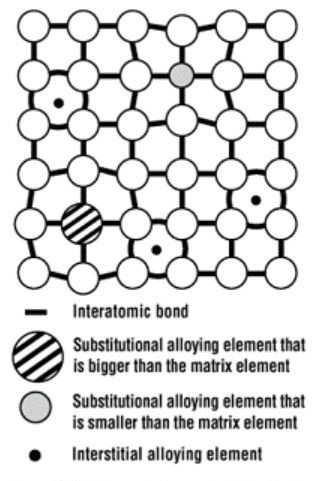
\includegraphics[width=.5\textwidth]{small_gaps_between_atoms.jpg}
    \caption{Small gaps between atoms, called “interstices” \cite{bajaj2020steels}.}
    \label{ch3:figure:gaps}
\end{figure}

Ferrite is a solid solution of iron, containing carbon, or one or more alloying elements, such as silicon, chromium, manganese, and nickel \cite{molabe2018determining}. In addition, it has an interstitial solid solution and a substitutional solid solution. Since the carbon elements have occupied the interstices, larger elements such as manganese, magnesium, silicon, and phosphorus substitute for iron in the lattice, see Figure \ref{ch3:figure:tank} \cite{jones2012engineering}. However, there is a limitation on how much carbon can occupy the interstices. Commonly, 0.02\% carbon at 725 ℃, but dropping to 0.006\% carbon at room temperature is more than enough to fit in the interstices \cite{bhadeshia2017steels}. Ferrite has a bcc crystal structure with a microstructural phase that is soft, ductile, which is similar to pure iron \cite{bajaj2020steels}. The microstructure of ferrite is shown in Figure \ref{ch3:figure:microstructure}.

\begin{figure}[H]
    \centering
    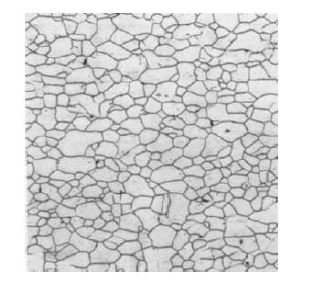
\includegraphics[width=.5\textwidth]{microstructure_of_carbon_steel.jpg}
    \caption{Microstructure of fully ferritic, ultralow carbon steel. Marshalls etch + HF, 300x \cite{molabe2018determining}.}
    \label{ch3:figure:microstructure}
\end{figure}

\subsection{Austenite} 
In the phase known as austenite, the interstices are much larger than in the ferrite phase and have the \acrshort{fcc} crystal structure, as shown in Figure \ref{ch3:figure:austenite} \cite{bajaj2020steels}. This allows more carbon content to occupy the interstices. At critical temperatures, which is around 1,150 ℃, carbon content up to 2\% can fit into the austenite, as the result of larger interstices \cite{bhadeshia2017steels}. As a consequence, in plain-carbon and low alloy steels, the austenite phase is not possible to form at room temperature but can only exist in relatively small amounts of retained austenite that was unable to transform during the rapid cooling process \cite{molabe2018determining}.

Since the austenite phase is not possible to form at room temperature for the lowest alloy steels, then their properties are also affected. Consequently, austenitic steels usually suffer from stress-corrosion cracking and low yield strength. Moreover, their strengthening processes are limited to only cold working, interstitial solid-concentrate strengthening, or precipitation hardening \cite{molabe2018determining}. However, \acrshort{fcc} alloy has low-temperature toughness, excellent weldability, and resistance to corrosion \cite{bhadeshia2017steels}.

 
\begin{figure}[H]
    \centering
    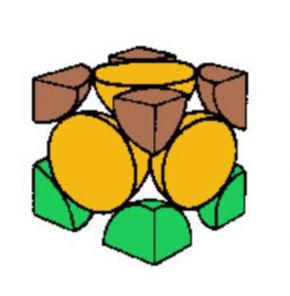
\includegraphics[width=.5\textwidth]{austenite_fcc_crystal_structure.jpg}
    \caption{An austenite FCC crystal structure \cite{bajaj2020steels}.}
    \label{ch3:figure:austenite}
\end{figure}

\subsection{Pearlite}
When the largest amount of carbon has occupied the interstices to form austenite at the critical temperature, the steel gradually cools at eutectoid temperature (723℃) on the iron-iron carbide equilibrium diagram, shown in Figure \ref{ch3:figure:equilibrium}. Thus, the carbon content is forced out of the concentrate  \cite{bhadeshia2017steels}. During this cooling process, the austenite transforms into a combination of ferrite and another phase known as cementite, also known as iron carbide, which has the chemical composition of Fe3C \cite{cmrp2014maintenance}. The combination of ferrite and cementite is known as \emph{pearlite}.

For plain carbon steels, ferrite, cementite, and pearlite phases are the principal constituents of the microstructure, provided that they have been cautiously subjected to slow cooling to avoid the formation of the metastable phases. Consequently, it is significant to evaluate the nucleation and growth of these phases and to determine the factors which control their morphology \cite{bhadeshia2017steels}.

\begin{figure}[H]
    \centering
    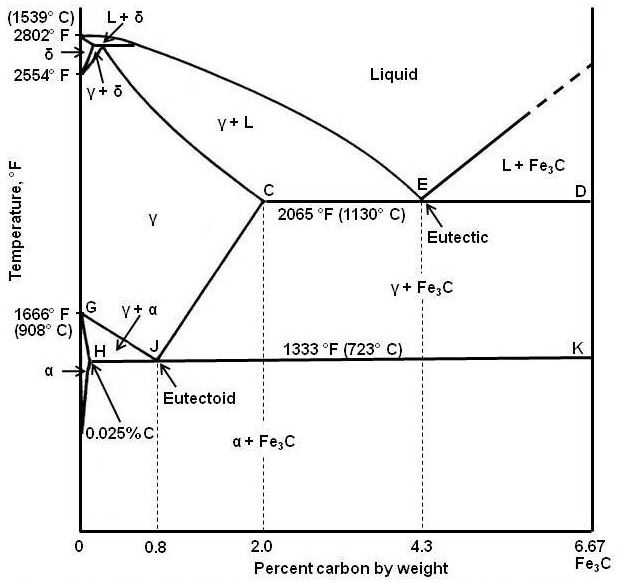
\includegraphics[width=\textwidth]{iron-iron_carbide_equilibrium_diagram.jpg}
    \caption{Iron-iron carbide equilibrium diagram showing the austenite ($\gamma$), ferrite ($\alpha$) and cementite (Fe3C) phase regions with eutectoid composition and temperature \cite{cmrp2014maintenance}.}
    \label{ch3:figure:equilibrium}
\end{figure}

Cementite on its own has characteristics of ceramic materials, very hard and brittle, with low toughness and little resistance to crack initiation and propagation, which is unlike ferrite \cite{bajaj2020steels} As a result, pearlite may reveal more than one microstructure due to the alternating layers of ferrite and cementite. A fully pearlitic microstructure is significantly formed at the eutectoid composition of 0.78\%C, as shown in Figure \ref{ch3:figure:equilibrium} \cite{molabe2018determining}. In contrast to cementite, fully pearlitic steels have high strength, high hardness, and good wear resistance. However, they commonly suffer from poor ductility and poor toughness \cite{molabe2018determining}. Figure \ref{ch3:figure:pearlite:microstructures} shows a microstructure fully pearlite steel and pearlite showing ferrite and cementite lamellae.

\begin{figure}[H]

\centering
\begin{subfigure}{.45\textwidth}
    \centering
    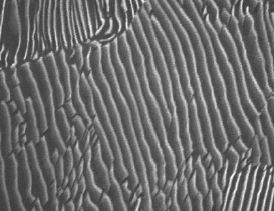
\includegraphics[height=5cm,width=\textwidth]{ferrite_and_cementite_lamellae_micrograph.jpg}
    \caption{}
\end{subfigure}
\begin{subfigure}{.45\textwidth}
    \centering
    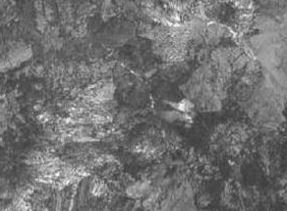
\includegraphics[height=5cm,width=\textwidth]{fully_pearlitic_steel.jpg}
    \caption{}
\end{subfigure}

\caption{Pearlite microstructures:  SEM micrograph of pearlite showing ferrite and cementite lamellae. 4\% picral etch. 10000x (a). Fully pearlitic steel showing the characteristic fine pearlite interlamellar spacing. 2\% nital + 4\% picral etch. 500x (b) \cite{molabe2018determining}.}
\label{ch3:figure:pearlite:microstructures}
\end{figure}

\subsection{Ferrite-Pearlite}
Ferrite-pearlite is the common microstructural phase that makes the plainest carbon steel. The microstructure and properties of these steels are distinguished, usually by the carbon content present and the size of the grains, as shown in Figure \ref{ch3:figure:austenite} \cite{molabe2018determining}. However, as previously stated in Section \ref{ch3:anchor:section:morphology}, carbon content has an impact on some properties of steel, thus it has a strong relationship with the tensile strength of ferrite-pearlite steels. As illustrated in Figure \ref{ch3:figure:properties}, carbon content has a direct relationship with the ultimate strength of ferrite-pearlite steels due to the gradual increase of ultimate tensile strength as a function of carbon content \cite{zhao2013effects}.

Pearlite has more carbon content on the microstructure, thus this is the main reason for the increase in the ultimate strength of ferrite-pearlite steels \cite{bajaj2020steels} Consequently, the strength of pearlite is much higher than that of ferrite \cite{molabe2018determining}. In contrast, the yield strength of ferrite-pearlite steels is not dependent upon the carbon content. However, the ferrite matrix commonly governs the yielding in ferrite-pearlite steels. The Ferrite matrix is regarded as a repeating phase in the microstructure of ferrite-pearlite, hence pearlite alone has a slight effect on the yielding behaviour \cite{molabe2018determining}. Figure \ref{ch3:figure:contents} shows the microstructure of ferrite-pearlite steels at two different carbon contents, to further understand the effect of carbon on steels.

\begin{figure}[H]

\centering
\begin{subfigure}{.45\textwidth}
    \centering
    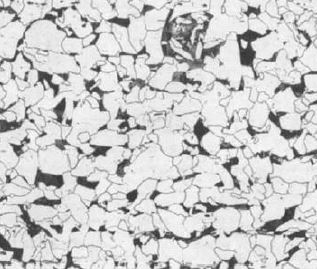
\includegraphics[height=.95\textwidth, width=\textwidth]{ferrite-pearlite_carbon_content_1.jpg}
    \caption{}
\end{subfigure}
\begin{subfigure}{.45\textwidth}
    \centering
    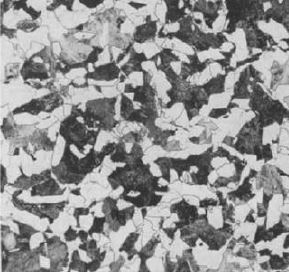
\includegraphics[height=.95\textwidth, width=\textwidth]{ferrite-pearlite_carbon_content_2.jpg}
    \caption{}
\end{subfigure}

\caption{Microstructure of typical ferrite-pearlite steels at two different carbon contents: a) 0.10\% C and b) 0.25\% C. 2\% nital + 4\% picral etch. 200x \cite{osei2015foam}.}
\label{ch3:figure:contents}
\end{figure}
 
\begin{figure}[H]
    \centering
    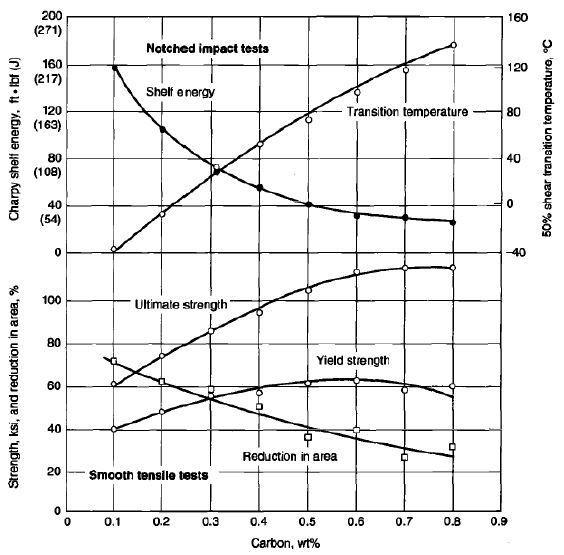
\includegraphics[width=.8\textwidth]{mechanical_properties_of_ferrite-pearlite_steels.jpg}
    \caption{Mechanical properties of ferrite-pearlite steels, as a function of carbon content \cite{molabe2018determining}. }
    \label{ch3:figure:properties}
\end{figure}

\subsection{Martensite}
Martensite is a supersaturated solid concentrate of carbon in iron \cite{molabe2018determining}. It is generally formed during the rapid cooling process when the waste carbon of the fcc austenite does not have time to diffuse out of the crystal structure and form cementite \cite{bajaj2020steels} Instead, the carbon content is 'trapped' in with the now almost pure iron, and is relatively forced into interstitial locations that are not large enough to accommodate the carbon atoms. Consequently, this distorts and strains the crystal matrix into a body-centred tetragonal (bct) structure, as shown in Figure \ref{ch3:figure:martensite}. Thus this forms a very hard phase known as martensite \cite{molabe2018determining}.
 
\begin{figure}[H]
    \centering
    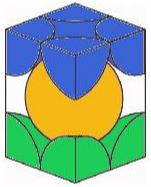
\includegraphics[width=.25\textwidth]{bct_crystal_structure_of_martensite.jpg}
    \caption{A bct crystal structure of martensite, which has larger gaps within the unit cell \cite{bajaj2020steels}.}
    \label{ch3:figure:martensite}
\end{figure}

When the content of carbon is constantly increasing to higher levels, more carbon is frozen into the bct structure, further straining the crystal matrix. Thus this is the main reason for the hardness of martensite to increase a function of carbon content \cite{bajaj2020steels} In addition, the volume of the bct martensite structure is larger than that of the fcc austenite. Consequently, the transformation of fresh martensite is significantly compressed by the surrounding matrix \cite{bajaj2020steels}. A typical microstructure of martensite is shown in Figure \ref{ch3:figure:martensite:microstructures}.

The hardness of martensite can be significantly reduced by further heating the martensite. In such cases, the carbon content has the opportunity to diffuse out from the bct structure, reducing the distortion of the crystal matrix in that process, and thus reducing the hardness and increasing the toughness \cite{bhadeshia2017steels}. However, after the heat treatment process, the microstructure of ferrite and iron carbide is formed, which leads to the formation of \emph{tempered martensite} \cite{bajaj2020steels}. Since the martensitic matrix is strained, it results in an increased amount of iron carbide nucleation sites in tempered martensite, which eventually leads to a more widespread distribution of iron carbide than seen in the lamellar (layered) structure of pearlite, shown in Figure \ref{ch3:figure:microstructure} \cite{bajaj2020steels} The bcc ferrite has a smaller volume compared to bct martensite, thus when martensite is tempered, some of the remaining martensite compression stresses from the austenite-to-martensite transition are mitigated \cite{molabe2018determining}.

\begin{figure}[H]
\centering

\begin{subfigure}{.45\textwidth}
    \centering
    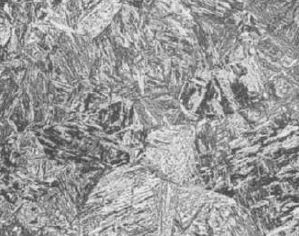
\includegraphics[height=6cm, width=\textwidth]{lath_martensite_microstructure.jpg}
    \caption{}
\end{subfigure}
\begin{subfigure}{.45\textwidth}
    \centering
    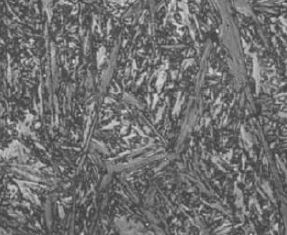
\includegraphics[height=6cm, width=\textwidth]{plate_martensite_microstructure.jpg}
    \caption{}
\end{subfigure}

\caption{Martensite microstructures: a) a typical lath martensite and b) a plate martensite. 4\% picral + HCl. 200x \cite{molabe2018determining}.}
\label{ch3:figure:martensite:microstructures}
\end{figure}

\subsection{Bainite}
Bainite is another possible microstructure that can form when austenite is cooled. It is typically a mixture of ferrite, cementite, and retained austenite. However, ferrite has an acicular morphology and the carbides are discrete particles, which is the main difference from the pearlite microstructure \cite{molabe2018determining}. \emph{Retained austenite} is the term given to austenite that does not transform to martensite during quenching \cite{bajaj2020steels} The cooling rate required to form bainite is much slower compared to the cooling rate needed to form martensite. As a consequence, carbon has the opportunity to diffuse out of the fcc austenite, thus allowing the formation of the \acrshort{bcc} ferrite.

Bainitic microstructures have an excellent balance in terms of strength and ductility, which is useful in many applications. These are the results of a sufficient cooling rate that significantly increases the strength. The higher cooling rates required to produce bainite give the harder components of the microstructure enough energy to transform into a more rounded shape \cite{bajaj2020steels}. In this way, the hard microstructural constituents do not easily suffer crack initiation and propagation as compared to flat and elongated ones.

Normally bainite has two morphologies, namely, upper bainite and lower bainite, which are shown in Figure \ref{ch3:figure:bainite:microstructures}. These two morphologies depend upon the temperature regions at which bainite was formed during the isothermal transformation \cite{molabe2018determining}. The upper bainite is typically formed isothermally in the temperature range of 400-550 ℃, while lower bainite is also formed by an isothermal process in the temperature range of 250-400 ℃ \cite{molabe2018determining}. Consequently, the iron carbide phase critically forms at the lath boundaries in upper bainite, while the carbide phase forms on certain crystallographic planes within the laths in lower bainite \cite{bajaj2020steels}. The lower bainite has higher strength and higher toughness compared to the upper bainite due to the fine acicular structure and the carbides within the laths. Generally, lower bainite has higher strength and higher toughness compared to upper bainite. This is due to the fine acicular structure and carbides possessed by lower bainite within the laths \cite{molabe2018determining}.
     
\begin{figure}[H]

\centering
\begin{subfigure}{.45\textwidth}
    \centering
    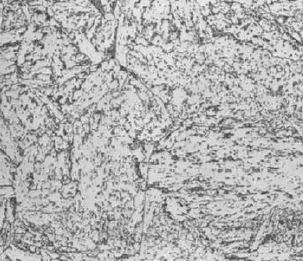
\includegraphics[height=.9\textwidth, width=\textwidth]{upper_bainite_microstruce.jpg}
    \caption{}
\end{subfigure}
\begin{subfigure}{.45\textwidth}
    \centering
    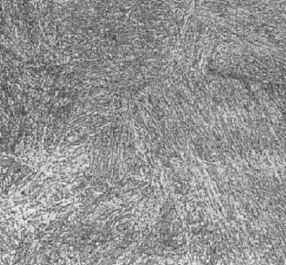
\includegraphics[height=.9\textwidth, width=\textwidth]{lower_bainite_microstructure.jpg}
    \caption{}
\end{subfigure}

\caption{Bainite microstructures: upper bainite (a) and lower bainite (b), in Cr-Mo-V rotor steel. 2\% nital + 4\% picral etch. 500x \cite{molabe2018determining}.}
\label{ch3:figure:bainite:microstructures}
\end{figure}

\subsection{Ferrite-Cementite}
When plain carbon steels are heated to temperatures slightly below the lower critical temperature, a ferrite-cementite microstructure that has a spheroidized shape as shown in Figure \ref{ch3:figure:spheroidized_steel} is significantly formed \cite{molabe2018determining}. However, the spheroidized structure is commonly revealed after the formation of pearlite. During the spheroidization, the cementite lamellae of the pearlite change their morphology to result to form spheroids \cite{molabe2018determining}.

The critical and controlling factors during this process are the The critical and controlling factors during this process are the diffusion of carbon and portions of lamellae that should significantly dissolve and then diffuse to yield the formation of a spheroid from the remaining portions of lamellae \cite{molabe2018determining}. The ferrite-pearlite phase has several benefits in terms of the resulting properties. For example, fully spheroidized structures normally have enhanced machinability properties for most plain carbon steels \cite{molabe2018determining}.  The machinability of steels is one of the vital properties in the present study thus the formation of ferrite-cementite should be thoroughly evaluated and assessed.

\begin{figure}[H]
    \centering
    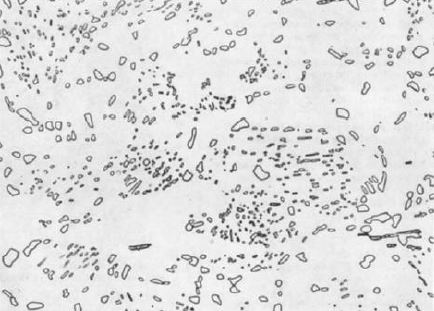
\includegraphics[width=.6\textwidth]{microstructure_of_fully_spheroidizel_steel.jpg}
    \caption{Microstructure of fully spheroidized steel. 4\% picral etch. 100x \cite{molabe2018determining}.}
    \label{ch3:figure:spheroidized_steel}
\end{figure}

\subsection{Ferrite-Austenite}
The ferrite-austenite are the two phases that are present in duplex stainless steels, see Figure \ref{ch3:figure:steel_phase}. The proportion of these two phases in duplex stainless steels in relatively equal. The duplex stainless steels can be altered to a completely ferritic structure. This is possible when they are melted and solidifies from the liquid phase \cite{xiao2006challenge}.  However, as the materials significantly cool to room temperature, about half of the ferritic grains transform into austenitic grains \cite{steels3practical}. Figure \ref{ch3:figure:duplex_microstructure} shows a combination of ferrite and austenite phases that forms one microstructure.

The combination of ferrite and austenite structures yields several attractive properties. Consequently, duplex stainless steels are about twice as stronger compared to regular austenitic and ferritic stainless steel \cite{steels3practical} The ductility of duplex steels is relatively fair, they, however, do not reach the excellent values of austenitic grades due to the different levels of nickel \cite{molabe2018determining}. Stress corrosion resistance is another property that has made duplex stainless steels to be the most extensively utilized family of stainless steels. 

\begin{figure}[H]
    \centering
    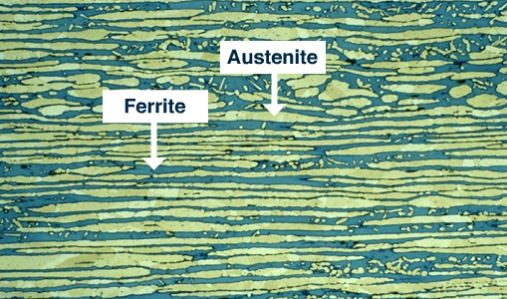
\includegraphics[width=.6\textwidth]{duplex_microstructure_that_has_yellow_austenitic_phase.jpg}
    \caption{Duplex microstructure that has yellow austenitic phase as “islands” surrounded by the blue ferritic phase \cite{steels3practical}.}
    \label{ch3:figure:duplex_microstructure}
\end{figure}

\section{Characterization of defects} 
While the microstructure of steels critically determines the resulting properties, they may still have a variety of imperfections known as defects and discontinuity. Both material discontinuity and crystal defects have diverse effects on the deformation behaviour and some of the physical and chemical properties of steels \cite{suryanarayana2017microstructure}. Hence it is of great significance to determine the nature and quantity of the crystal defects present in a steel material. 

Numerous methods have been extensively utilized to characterize the defects in steel. However, according to some researchers, the \Acrfull{tem} technique is more suitable to characterize defects on steels \cite{george2002introduction, bhadeshia2017steels}. Besides, the \acrshort{tem} method has been proven to be reliable on numerous occasions. In any metallic material crystal defects can occur, these defects may include, point defects (vacancies, interstitial atoms), line defects (dislocations), planar defects (stacking faults, twin boundaries), and volume defects (voids, cavities). One of the objectives of the present study is to improve the properties of steels based on the understanding of microstructure morphology. Thus, the characterization of vacancies and dislocation defects is also of interest.

\subsection{Vacancies} 
 In almost every instance, individual vacancies cannot be seen on \acrshort{tem}, due to the size and complications that are usually encountered. However, their aggregation into voids, resulting in the formation of dislocation loops in quenched steels, helps in estimating the vacancy concentration. In this way, the dislocation loops are significantly characterised, which then makes it possible to determine whether they are formed from vacancy condensation or interstitial atoms \cite{suryanarayana2017microstructure}.

\subsection{Dislocations}
This defect is commonly divided into two types, screw and edge dislocation. The complications arise when characterizing the type of dislocation that is present in steels \cite{jones2012engineering}. However, this is conveniently achieved by using the extinction (invisibility) criterion \textbf{g.b} = 0, where \textbf{g} is the reciprocal lattice vector, and \textbf{b} is the burgers vector. By properly orientating the specimen, a dislocation will become invisible, and this can occur at more than one \textbf{g} value. The equation can nonetheless be manipulated by simply putting the determination of two (or more) of these \textbf{g} values, which then enables calculating \textbf{b} \cite{suryanarayana2017microstructure}.

Many experimental studies have been conducted to ease and improve the characterization of crystal defects \cite{george2002introduction, bhadeshia2017steels, karayan2014weld}. Despite this, Suryanarayana \cite{suryanarayana2017microstructure} validated that \acrshort{tem} remains a suitable technique for characterizing crystal defects in steels. Moreover, \acrshort{tem} enables the determination of disorientation between grains (for both low-angle and high-angle grain boundaries), the fault vector in stacking faults, the extent of coherency, or incoherency between two phases, the sizes and volume fractions of precipitates, and many other features \cite{suryanarayana2017microstructure}.

\section{Effects of heat treatment on steels}
\label{ch3:anchor:section:treatment}
Heat treatment is an industrial process that is commonly used to improve the existing properties of metals, especially steels. To be precise, it is often used to enhance mechanical, physical, and sometimes chemical properties \cite{mampuya2021effect}. The heat treatment process modifies the microstructure of the steel, thus altering the resulting properties. The role of each microstructural constituent is comprehensively presented in Figure \ref{appendix:role} on appendices. In recent years several methods have been developed to enhance the properties of engineering materials, especially for liquid storage facilities. Approaches like thermochemical and thermomechanical are examples of such techniques \cite{singh2020applied}. However, the heat treatment process has been a sensible approach for the optimization of steel properties.

Normally, the first step in the heat treatment of steel is to effectively heat the steel to some temperature at or above the critical range to form austenite \cite{mampuya2021effect}. However, to fully comprehend the heat treatment process of steels, it is crucial to first understand the phase diagram for the steel of interest. Heat treatment comprises several subsequent processes that are all critical. Various heat treatments are normally based on the subsequent cooling and reheating of the austenitized steel \cite{singh2020applied}.  For the present research work, only the relevant heat treatment processes will be discussed.

\subsection{Annealing}
The ductility of steel or any metallic material is normally enhanced by the annealing process. This process involves heating the steel to a predetermined temperature and then slowly cooling it to room temperature in a furnace \cite{singh2020applied}. However, enhancing the ductility of the steel results in a reduction in brittleness. Sometimes annealing process can be utilized to improve the machinability of steels \cite{nikkhah2019improved}. As a consequence, annealing is a vital process for liquid storage facilities due to the demand for ductility and ease of machinability during the fabrication process. The full annealing temperature cycle is shown in Figure \ref{appendix:range} on appendices, which includes the hardness range on steel after annealing. 

Annealing is a broad process that involves several thermal cycles, which are classified based on the maximum level of temperature reached during the heating of the steel \cite{singh2020applied}. The thermal cycles usually involve subcritical, inter critical, and full annealing. Appendix 2.1 indicates the recommended temperatures and cooling cycle for full annealing of various carbon steel forgings \cite{singh2020applied}.

\subsection{Normalizing}
The purpose of normalizing is very broad and normally depends upon the history of the steel, the cycle of heating, and cooling practised. However, this process is commonly used to achieve the desired hardness and strength of the steel \cite{singh2020applied}. Therefore, it can increase or decrease these properties, depending on the objectives. 

Normalizing is sometimes known for overlapping the function of other types of heat treatments, such as annealing, hardening, and stress relieving \cite{singh2020applied}. This is due to multiple properties it normally improves simultaneously, which can be individually achieved by each other heat treatment processes. Normalising can produce harder and stronger steel and also improves machinability \cite{mampuya2021effect}. However, in the normalizing process, the cooling is not performed under equilibrium conditions, thus there are often deviations from the phase diagram predicted structures \cite{singh2020applied}.  For steels that are normally used for the construction of liquid storage facilities, normalizing is essential to achieve the desired strength and hardness, as well as improved machinability.

\subsection{Tempering}  
Almost all steels are too brittle in the quenched martensitic condition for most applications, especially storage facilities. This is due to high residual stresses that are commonly induced as the result of martensite transformation \cite{mampuya2021effect}. Consequently, tempering always follows the hardening or normalizing process to relieve the residual stresses and relax the steel. 

Tempering is a heat treatment process that involves heating the steel to a temperature below the lower critical temperature \cite{singh2020applied}. This results in relieving the residual stresses, and enhancement of the ductility and toughness of the steel. In most heat treatment processes, there is usually a sacrifice of other properties to obtain others. As a consequence, in the tempering process, there is a sacrifice of hardness and strength. As the tempering temperature is constantly increased, the hardness decreases, while the toughness increases \cite{singh2020applied}. Various types of tempering are known to date, austempering and martempering are the commonly used processes.

\subsection{Quenching}  
The rate of cooling of any metallic material is vital and has an impact on the resulting properties. Quenching is the process of cooling the steel, usually at a rapid rate, to produce a martensitic transformation \cite{singh2020applied}. The rate of cooling has different effects on different metals, in ferrous alloys, the rapid rate will result in a harder metal, while in non-ferrous alloys, a softer metal will be produced \cite{mampuya2021effect}. The rapid rate of cooling usually hardens steel. Therefore, in order to achieve softer steel, a slower rate of cooling should be applied. However, this, of course, varies with the type of steel. 

Quenching can be achieved in numerous ways, commonly by forced air or other types of gases. Liquids such as water and oil can also be utilized to quench steels due to their better thermal conductivity \cite{singh2020applied}. There are three stages of cooling during the quenching process, and all are closely related to the cooling medium being used. Vapour is the first quenching medium that is applied to the steel surface, and during this stage, the cooling process is relatively slow. When the metal has cooled enough, and the vapour film is no longer stable, the second stage then takes place, which is wetting the surface of the steel. This is usually the rapid stage of cooling the steel. Finally, liquid cooling commences when the surface temperature of the steel finally reaches the boiling point of the liquid to halt the formation of vapour \cite{marzorati2018green, protopopoff2011surface}. However, this is commonly the slowest stage of cooling.

Recently, most researchers have been interested in understanding the relationship between heat treatments, microstructure, and mechanical properties \cite{marzorati2018green, whitman1924effect, cai2018influence}. Mampuya et al. \cite{mampuya2021effect} investigated the effect of heat treatment on the microstructure of duplex stainless steel 2205. They further reported that the transition of austenite and ferritic phases often results in critical changes in the hardness of the specimen when air-cooled. While there is a slight change in the hardness when it is water or oil-cooled. Ding et al. \cite{zhang2021influence} conducted an experimental study to understand the effect of slow-cooling heat treatment on the mechanical properties of high-strength steels. Their results indicated that the slow-cooling heat treatment can effectively reduce the yield and ultimate strengths of high-strength steels. Essoussi et al. \cite{essoussi2019heat} reported that the strength and elongation of AISI 304 austenitic stainless steels can be improved by quenching without tempering, while the hardness will relatively decrease during this process.

There is a lack of research on the effect of heat treatment on the corrosion properties of steel. However, some researchers have made a significant effort to thoroughly understand the relationship between corrosion and heat treatment processes \cite{whitman1924effect, hackerman1987theory}. The corrosion resistance of steel is largely dependent upon the composition and microstructures \cite{wang2020enhancing}. The microstructures could nonetheless be improved by the process of heat treatment. Sarkar et al. \cite{sarkar2020effects} investigated the effect of heat treatment on the microstructure, mechanical, and corrosion properties of stainless steel. The study showed that the retained austenite is more for specimens without solution annealing, which increases the tensile strain and decreases the hardness and wear rate. To enhance the corrosion resistance of martensite stainless steel, Wang et al. \cite{wang2020enhancing} conducted numerous experiments and they reported that the austenite phase disappears and new duplex particles accelerated after concentrate treatment and aging treatment, which decreased the pitting corrosion. 

One of the objectives of the present research work is to improve the corrosion resistance of duplex stainless and mild steels in a corrosive atmosphere. Consequently, all these previous studies and relevant literature is used as a benchmark for the present study. Experimentally and theoretically, they provide comprehensive guidance in terms of optimizing the materials used for constructing \acrshort{afff} storage facilities.

\section{Polyethylene plastics}
Plastics also known as polymers have become a major class of engineering materials. Polymers are substances whose molecules have high molar masses and are composed of a relatively large number of repeating units. There are both naturally occurring and synthetic polymers \cite{roslan2013effect}. They offer several beneficial properties (mechanical, physical, chemical and optical) when utilised for certain industrial applications \cite{nugent2017rotational}. In contrast to metals, polymers are generally characterised by lower density, strength, elastic modulus, thermal and electrical conductivity, high corrosion resistance, and cost \cite{roslan2013effect}. Thus, this is the reason for the rapid increase in plastic processing on annual basis. In addition, they are the preferred materials over metals nowadays for numerous industrial applications. However, their setback to date is they are a waste that affects the environment if no longer in use. Nonetheless, there have been developments over the years that are aiming to rectify this issue, with the notable one being recycling.  

Many plastic materials fall under the polymer tree. However, for the present study polyethene (\acrshort{pe}) plastics will be discussed. This is due to the growing demand for this material for manufacturing liquid storage facilities. \acrshort{pe} is undoubtedly the most popular plastic material in the world. It is a commodity material, which statically accounts for about 70\% of the plastic family \cite{roslan2013effect}.  \acrshort{pe} is thermoplastic in nature and therefore it can be reprocessed repeatedly, thus this is the reason it is easily available at a relatively low cost and can be easily processed \cite{kurtz2009cross}. Moreover, it can be utilised for diverse industrial applications. 

\acrshort{pe} is often classed by the density it contains. Therefore, there is a \Acrfull{ldpe} ($0.910 < density < 0.925$), \Acrfull{mdpe} ($0.926 < density < 0.940$), and \Acrfull{hdpe} \cite{gabriel1998history}. Consequently, changing the density of the \acrshort{pe} will result in altering the properties. The effect of changes in density, melt index, and molecular weight distribution on the properties of \acrshort{pe} are tabulated in Figure \ref{appendix:classifications} on appendices.

\acrshort{hdpe} is commonly used in the manufacturing of chemical or liquid storage facilities, due to the seamless final product that is produced, for greater strength and corrosion resistance, thus it is of great importance in the present study. \acrshort{hdpe} is a thermoplastic material composed of mainly carbon and hydrogen atoms joined together to form a high molecular weight product as shown in Figure \ref{ch3:figure:molecular_chains} \cite{gabriel1998history}. Methane gas is converted into ethylene then, with the application of heat and pressure it is further converted to polyethene. The polymer chain may be 500,000 to 1,000,000 carbon units long. The longer the main chain, the great the number of atoms \cite{gabriel1998history}. As expected, the properties of \acrshort{hdpe} or any plastic material depend upon the arrangement of the molecular chains.
               
\begin{figure}[H]
\centering

\begin{subfigure}{.3\textwidth}
    \centering
    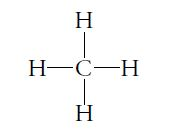
\includegraphics[width=\textwidth]{methane_molecular_chain.jpg}
    \caption{Methane}
\end{subfigure}
\begin{subfigure}{.3\textwidth}
    \centering
    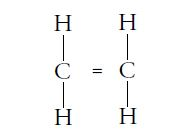
\includegraphics[width=\textwidth]{ethylene_molecular_chain.jpg}
    \caption{Ethylene}
\end{subfigure}
\begin{subfigure}{.65\textwidth}
    \vspace{1.5em}
    \centering
    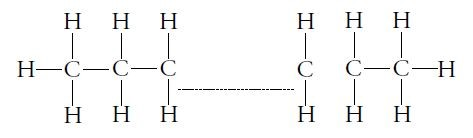
\includegraphics[width=\textwidth]{polythylene_molecular_chain.jpg}
    \caption{Polyethylene molecular chain}
\end{subfigure}

\caption{a) Methane gas, b) ethylene and c) polyethylene \cite{gabriel1998history}.}
\label{ch3:figure:molecular_chains}
\end{figure}

\subsection{Cross-linked polyethylene (XLPE) material}
Many researchers have been making efforts in obtaining a \acrshort{pe} with specific chemical, mechanical, and thermal characteristics for the fabrication of complex-shaped products, or for use in adverse environmental conditions \cite{kurtz2009cross}. In general, plastic is a light and weak substance that easily melts when exposed to heat. However, altering the carbon atoms within the structure changes this perspective. To be precise, cross-linking the carbon atoms within the structure usually transforms such material into a superior material that may be resistant to temperature, pressure, and corrosion, and that can be used in a variety of applications \cite{peacock2000handbook}. Crosslinking is known as a process in which carbon atoms of the same or different polyethene chains are joined together to form a three-dimensional network structure \cite{kurtz2009cross}.

The crosslinking technique was first discovered in the late 1960s by the European scientist known as Engel \cite{peacock2000handbook}. The introduction of cross-linked polyethene (\acrshort{xlpe}) was another milestone in the plastic era. As a consequence, when \acrshort{pe} is cross-linked, it is advantageously employed in the manufacturing of storage facilities due to the advanced resulting properties. The fundamental way to enhance material properties such as impact strength, chemical resistance, and thermal characteristics is via cross-linking \cite{andreopoulos1986mechanical}. Cross-linking will however change the nature of the polymer from thermoplastic to thermosetting polymer, thus yielding a non-melting and more durable polymer matrix \cite{clemens2017microstructure}. Crosslinking method is easily achieved in branched polymers. From the branched \acrshort{hdpe} it is convenient to crosslink the polymer. However, this is a long and tiring process as compared to \acrshort{ldpe}.

Since \acrshort{hdpe} has a linear molecular structure, therefore crosslinking this type of polymer requires special attention as compared to \acrshort{ldpe}. Figure \ref{ch3:figure:hdpe} and \ref{ch3:figure:ldpe} shows the process of branching \acrshort{hdpe} and \acrshort{ldpe} respectively.
 
\begin{figure}[H]
    \centering
    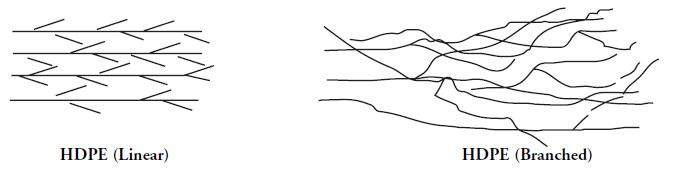
\includegraphics[width=\textwidth]{linear_and_branched_hdpe.jpg}
    \caption{Linear and branched HDPE \cite{gabriel1998history}.}
    \label{ch3:figure:hdpe}
\end{figure}

\begin{figure}[H]
    \centering
    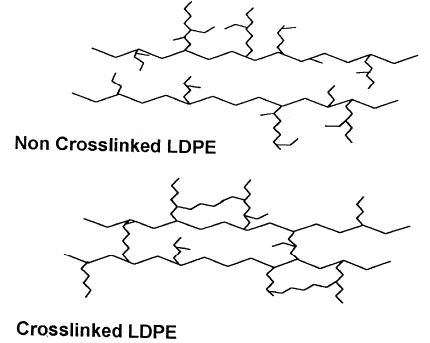
\includegraphics[width=.6\textwidth]{crosslinked_and_non_crosslinked_ldpe.jpg}
    \caption{Crosslinked and non-crosslinked LDPE. \cite{kurtz2009cross}.}
    \label{ch3:figure:ldpe}
\end{figure}

Over the past decades, there have several crosslinking methods that have been developed. However, to date, two tested methods are used to crosslink polymers, chemical and radiation (physical) methods \cite{clemens2017microstructure, bajaj2020steels}. These two methods are unique in their way and are often utilized for a specific purpose. They usually depend upon the state (molten or solid) of the polymer during crosslinking and the type of activator used to promote crosslinking \cite{kurtz2009cross}. Figure \ref{ch3:figure:crosslinking_methods} illustrates the available crosslinked methods in detail, as discussed above.

\begin{figure}[H]
    \centering
    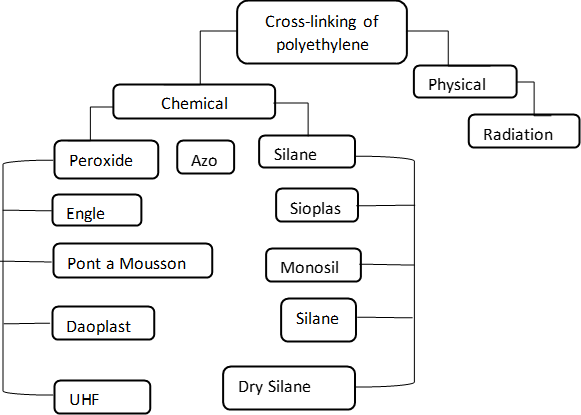
\includegraphics[width=.75\textwidth]{methods_available_for_crosslinking_polyethylene.png}
    \caption{Methods available for crosslinking polyethylene \cite{patterson2022cross}.}
    \label{ch3:figure:crosslinking_methods}
\end{figure}

\subsubsection{Chemical processes}
This is an extensively used method for crosslinking polymers. For the method to work as desired, a chemical substance usually peroxide or silane is required to significantly activate the links in the polymer chain, thus it is known as a chemical process \cite{peacock2000handbook}. During the chemical process, crosslinking takes place through direct carbon-to-carbon bonds. An alternative may be through the chemical bridges that connect various polyethene molecules \cite{kurtz2009cross}. 

In recent years, most researchers have been interested in knowing the crosslinking method that yields quality thermoplastic. The recent relevant literature suggests that the intensity of crosslinking in thermoplastic resin usually varies with the crosslinking process. Chemical crosslinking using peroxide significantly results in the highest and most uniform degree of crosslinking as compared to the radiation process \cite{clemens2017microstructure, bajaj2020steels}. Tamboli et al. \cite{peacock2000handbook} experimentally investigated the difference in the degree of crosslinking polymers using chemical and radiation processes. The outcome was that radiation crosslinking yields between 34-75\% degree of crosslinking. In the chemical crosslinking method, peroxide gives a much higher degree of crosslinking (up to 90\%), while silane-based crosslinking can be 45-70\% degree of crosslinking.

\paragraph{Peroxide processes} \hfill \\
Peroxide crosslinking process has been utilised for nearly over 40 years and is the most common crosslinking process of thermoplastics, especially polyethene. In this method, the organic peroxide is used as the initiator. In most cases, an organic peroxide is used its original unprocessed structure \cite{peacock2000handbook}. It is important to note that this process only occurs when the thermoplastic is in a molten state. In addition, the process is a carbon-based chemical that includes a minimum of two oxygen atoms that are bonded together (-O-O-). The general formula is:

 \begin{equation}
    R^1-O-O-R^2
 \end{equation}

Where, R1 and R2 values can be aryl, alkyl, or acyl groups and O being the two oxygen atoms which are bonded together. The alkyl peroxides significantly produce the most reactive free radicals; thus, they are the most used peroxides for crosslinking \cite{kurtz2009cross}. Figure \ref{ch3:figure:crosslinking_process} shows the entire schematic representation of crosslinking polyethene using the peroxide substance. The peroxide process has the advantage of producing high thermal stability products due to the C-C bonds, however, this is achieved at relatively high costs \cite{patterson2022cross}.

\begin{figure}[H]
    \centering
    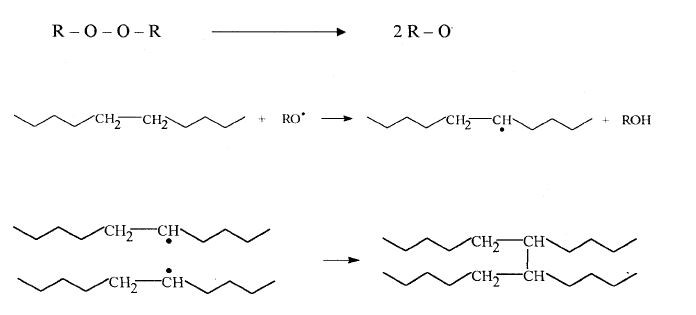
\includegraphics[width=.9\textwidth]{process_of_crosslinking_using_the_organic_peroxide_as_the_initiator.jpg}
    \caption{Process of crosslinking using the organic peroxide as the initiator \cite{peacock2000handbook}. }
    \label{ch3:figure:crosslinking_process}
\end{figure}

\paragraph{Silane processes} \hfill \\
For this process to be possible, crosslinking is significantly activated by silane coupling agents, which react with many chemicals, including polymers, through typical organic chemistry reactions. The organ silane molecule critically includes a central silicon atom (Si) bounded to two different categories of groups (vinyl and alkoxy), which usually displays different reactivity \cite{kurtz2009cross}. Both these groups are vital in the process of cross-linking. The vinyl groups usually allow silane grafting to the \acrshort{pe} and alkoxy groups generate a three-dimensional network of siloxane linkages in the presence of water or moisture (through condensation or hydrolysis).

In contrast to the peroxide process, the \acrshort{pe} is cross-linked in the crystalline state in the silane process. Thus, the uses of silanes result in the formation of siloxane (Si-O-Si) bridges, which are less rigid than carbon-to-carbon (C-C) bonds produced in the peroxide process. The silane process is shown in Figure \ref{ch3:figure:reaction} in a two-step process, starting from the grafting of silane on \acrshort{pe} to condensation (cross-linking). At first, silane is grafted on \acrshort{pe}, then the condensation takes place yielding in cross-linking. One of the advantages of the silane process is that it can be achieved at room temperature and a relatively low cost.

\begin{figure}[H]
\captionsetup[subfigure]{justification=raggedright}
\centering

\begin{subfigure}{.9\textwidth}
    \centering
    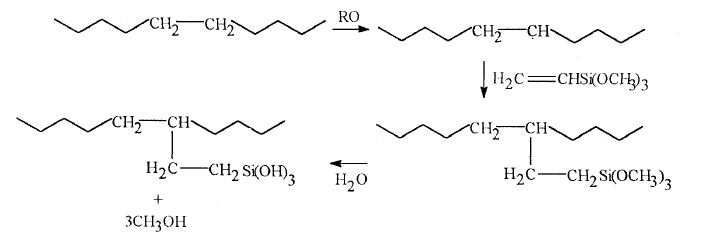
\includegraphics[width=\textwidth]{grafting_of_silane_on_pe.jpg}
    \caption{Grafting of silane on PE}
\end{subfigure}
\begin{subfigure}{.9\textwidth}
    \vspace{1.2em}
    \centering
    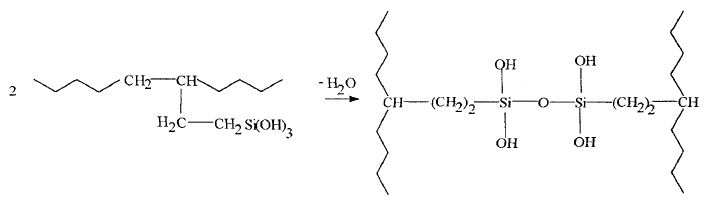
\includegraphics[width=\textwidth]{condensation.jpg}
    \caption{Condensation (crosslinking)}
\end{subfigure}

\caption{Silane grafted polyethylene crosslinking reaction \cite{kurtz2009cross}.}
\label{ch3:figure:reaction}
\end{figure}

\paragraph{Radiation (physical) processes} \hfill \\
In contrast to chemical processes, radiation processes do not necessarily require any addition of any sort of chemicals in the original compound of \acrshort{pe}. In the radiation method, crosslinking is significantly achieved by the free radical mechanism, which is generated in a radiation polymer chain using high energy \cite{peacock2000handbook}. As a consequence, two or more chains will join together where the free radical is generated. Figure \ref{ch3:figure:radiation} shows a schematic process of crosslinking \acrshort{pe} by radiation.

The involvement of high energy radiation on polymeric materials can critically produce crosslinking or cause a degradation in the main chain, which is termed ‘scission’ \cite{meola2005cross}. In this way, both chain scission and crosslinking occur simultaneously and competitively. However, the dominance of one or the other may significantly depend upon several factors such as the sensitivity of the polymer to radiation, irradiation dose, and polymer radiation environment \cite{meola2005cross}. To be precise, in the presence of oxygen (O2) scission is relatively dominant over crosslinking, while in an environment that contains other gases such as nitrogen (Ni), crosslinking is normally dominant \cite{peacock2000handbook}. However, the changes and chemical properties of the finished product depend mostly on the efficiency of the crosslinking reaction and its relative ratio with degradation \cite{meola2005cross}. For \acrshort{afff} storage facilities chemical properties of the cross-linked polymer are of great importance. This is due to the uses of \acrshort{afff}, as its chemical composition should not be influenced by the holding storage facility.

\begin{figure}[H]
\captionsetup[subfigure]{justification=raggedright}

\centering

\begin{subfigure}{.9\textwidth}
    \centering
    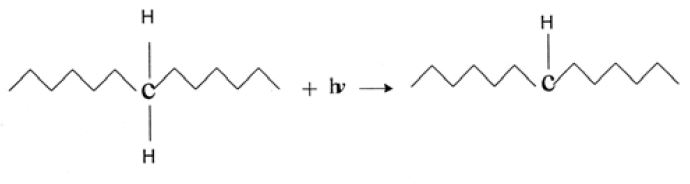
\includegraphics[width=\textwidth]{polyethylene_energy_radiation.jpg}
    \caption{}
\end{subfigure}
\begin{subfigure}{.9\textwidth}
    \centering
    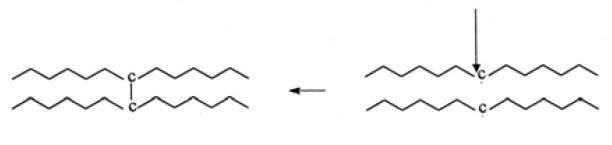
\includegraphics[width=\textwidth]{resulting_crosslinked_pe.jpg}
    \caption{}
\end{subfigure}

\caption{Polyethylene energy radiation (a) and the resulting crosslinked PE (b) \cite{peacock2000handbook}.}
\label{ch3:figure:radiation}
\end{figure}

Mathematically, the scission and crosslinking can be related in order to estimate the probability between them. This probability can be expressed as a ratio that is given by the following equation.

\begin{equation}
    \frac{\beta}{\alpha}=\frac{1}{2}\frac{G(S)}{G(X)}
\end{equation}

\begin{doublespace}
\noindent Where, \\
$\alpha\ is\ a\ probability\ of\ crosslinking\ of\ chains\ after\ one\ electron\ volt\ of\ energy\ absorbed.$ \\
$\beta\ is\ a\ probability\ of\ chain\ scission\ after\ one\ electron\ volt\ of\ energy\ absorded.$ \\
$G(X)\ is\ a\ number\ of\ crosslinking\ per\ 100eV\ of\ radiant\ energy\ absorbed.$ \\
$G(S)\ is\ a\ number\ of\ scission\ per 100eV\ of\ energy\ absorbed.$ \\
\end{doublespace}

The typical G(X) and G(S) values are listed in Table \ref{appendix:classifications} on appendices. \\

According to several scientists the bond energy for breaking of C-H bond is typically 364Kj/mol \cite{peacock2000handbook}. Therefore, the electron beam having sufficient energy to break C-H bond is normally suitable for crosslinking rather than scission \cite{peacock2000handbook}. The technique of crosslinking \acrshort{pe} by radiation normally involves the four main variables. 

\begin{itemize}
    \item The type of radiation and its sources.
    \item The nature of \acrshort{pe} structure to irradiated.
    \item Mechanism and theories of reaction.
    \item The properties of the network formation, especially physical, chemical, and mechanical. 
\end{itemize}

\subsection{Environmental Stress Crack Resistance (ESCR)}
\acrshort{afff} concentrate contains sensitive chemicals within its composition. Therefore, under certain temperature and stress conditions, the \acrshort{pe} material may begin to crack sooner than expected due to the presence of chemicals contained in the \acrshort{afff} concentrate. It has been experimentally proven that storage facilities containing chemically free liquids do not suffer from cracks as much as those containing chemical liquids. This phenomenon is known as the environmental stress crack (ESC). One of the objectives of the present work is to assess and evaluate the chemical resistance of \acrshort{hdpe} in the presence of \acrshort{afff} concentrate. The test methods that are usually utilised to evaluate ESC and other substances are provided in Figure \ref{appendix:classifications} in the appendices. 

All engineering materials that are suitable for storing liquids containing chemicals are critically evaluated against ECS. For \acrshort{pe}, normally the stress-cracking agents are polar materials such as alcohols, detergents, halogens and aromatics \cite{gabriel1998history}. \acrshort{afff} may be thought of as a detergent due to the bubbles it creates during utilisation. Consequently, it causes problems for \acrshort{pe} polymers. The property of a material to resist ESC is called environmental stress crack resistance (ESCR) \cite{gabriel1998history}. Researchers have been working on understanding the mechanism of ESCR, however, to date it is not entirely understood. In most instances, failures of \acrshort{pe} polymers that are caused by ESC tend to be due to the development of cracks in area tensile stress which gradually grow and propagate over time \cite{peacock2000handbook}.

Over the past years, there have been several efforts made in order to avoid ESC. Therefore, using an appropriate resin formulations of ESCR materials, designing the geometric appropriately, carefully using the manufacturing controls that prevents occurrence of severe stress risers, and limiting stresses and strains during the storage facility installation, all these are usually sufficient to avoid ESC \cite{gabriel1998history}. Moreover, \acrshort{pe} polymer may be cross-linked to improve the chemical properties and thus resist cracking.  With this regard, it is vital to test the compatibility of \acrshort{pe}, especially \acrshort{xlpe} with \acrshort{afff} concentrate in order to avoid unexpected circumstances during fire conditions. To date, there are over 40 different ESCR test methods that are used to determine the chemical resistance of various materials. The standard test that is currently used in the industry of polyethylene is bent-strip test \cite{gabriel1998history}. The method is normally used to assess the performance of polyethylene cable insulation but can be cautiously used to evaluate the performance of \acrshort{xlpe} storage facilities in the presence of \acrshort{afff} concentrate. The bent-strip test is shown in Figure \ref{ch3:figure:bending_apparatus}. Where the specimen is immersed into a surfactant of interest, and the time to failure is noted. The results are reported using the notation $F_{xx}$, where xx is the percentage of samples that has been tested.
 
\begin{figure}[H]
    \centering
    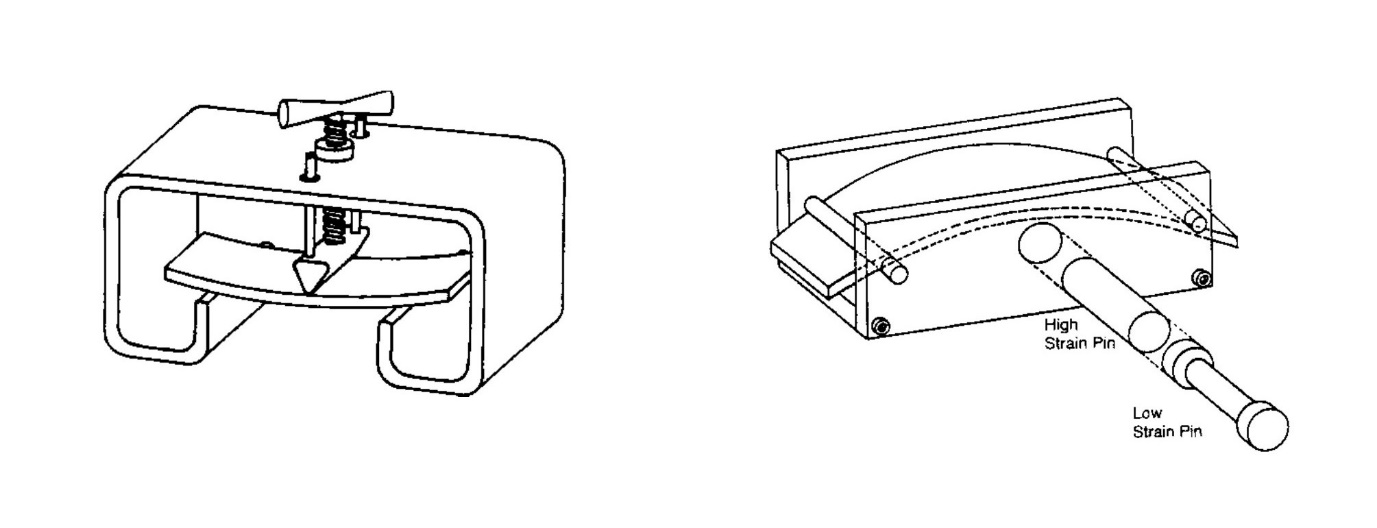
\includegraphics[width=.8\textwidth]{three_point_bending_apparatus_for_testing_escr.jpg}
    \caption{Three point bending apparatus for testing ESCR under constant strain \cite{choi2009modeling}.}
    \label{ch3:figure:bending_apparatus}
\end{figure}

Research shows that the density of the \acrshort{pe} polymer plays a critical role towards ESCR. For \acrshort{pe} resins of the same molecular weight, the lesser the density, the greater the ESCR. The greater the proportion of crystals, the greater the density and the brittleness of the resin, which causes a rapid crack initiation \cite{gabriel1998history}. However, since the phenomenon of ESC is not fully understood, then the density alone is inadequate to predict the ESCS.

\section{Conclusion}
This chapter discussed the engineering materials investigated in the present study. Both metals and plastics materials were closely assessed. The previous research was studied; this was used as a benchmark in this research. The atomic bonding, cross-linking methods, properties of interest, microstructure, and heat treatment processes are investigated. The properties of most materials depend upon the microstructure. Consequently, heat treatment processes are vital when improving these properties to better store \acrshort{afff} concentrate.

\acrshort{pe} plastics are rapidly replacing metals nowadays. They have several advantages over metal, as they are light in weight, resistant to corrosion, durable, and relatively affordable. These plastics are often classified by the density they possess. In this chapter, the environmental stress-cracking resistance of these plastics was discussed. To alter the properties of \acrshort{pe}, a cross-linking method was opted for. To date, this is an effective method to avoid the phenomenon of ESC.

The next chapter discusses and compares the various methods of constructing storage facilities for \acrshort{afff} concentrate. The methods used to test the compliance of these storage facilities are discussed. Both national and international design standards are considered.